% -*- compile-command: "make HOCKING-PeakSegFPOP-pipeline-slides.pdf" -*-
\documentclass{beamer}
\usepackage{tikz}
\usepackage[all]{xy}
\usepackage{amsmath,amssymb}
\usepackage{hyperref}
\usepackage{graphicx}
\usepackage{algorithmic}

\DeclareMathOperator*{\argmin}{arg\,min}
\DeclareMathOperator*{\Lik}{Lik}
\DeclareMathOperator*{\PoissonLoss}{PoissonLoss}
\DeclareMathOperator*{\Peaks}{Peaks}
\DeclareMathOperator*{\Segments}{Segments}
\DeclareMathOperator*{\argmax}{arg\,max}
\DeclareMathOperator*{\maximize}{maximize}
\DeclareMathOperator*{\minimize}{minimize}
\newcommand{\sign}{\operatorname{sign}}
\newcommand{\RR}{\mathbb R}
\newcommand{\ZZ}{\mathbb Z}
\newcommand{\NN}{\mathbb N}

% Set transparency of non-highlighted sections in the table of
% contents slide.
\setbeamertemplate{section in toc shaded}[default][100]
\AtBeginSection[]
{
  \setbeamercolor{section in toc}{fg=red} 
  \setbeamercolor{section in toc shaded}{fg=black} 
  \begin{frame}
    \tableofcontents[currentsection]
  \end{frame}
}

\begin{document}

\title{Genome-wide supervised ChIP-seq peak detection}

\author{
  Toby Dylan Hocking\\
  toby.hocking@mail.mcgill.ca\\
  joint work with Guillem Rigaill, Paul Fearnhead, 
  Guillaume Bourque}


\date{26 Jan 2017}

\maketitle

\section{Problem: optimizing ChIP-seq peak detection}

\begin{frame}
  \frametitle{Chromatin immunoprecipitation sequencing (ChIP-seq)}
  Analysis of DNA-protein interactions.

  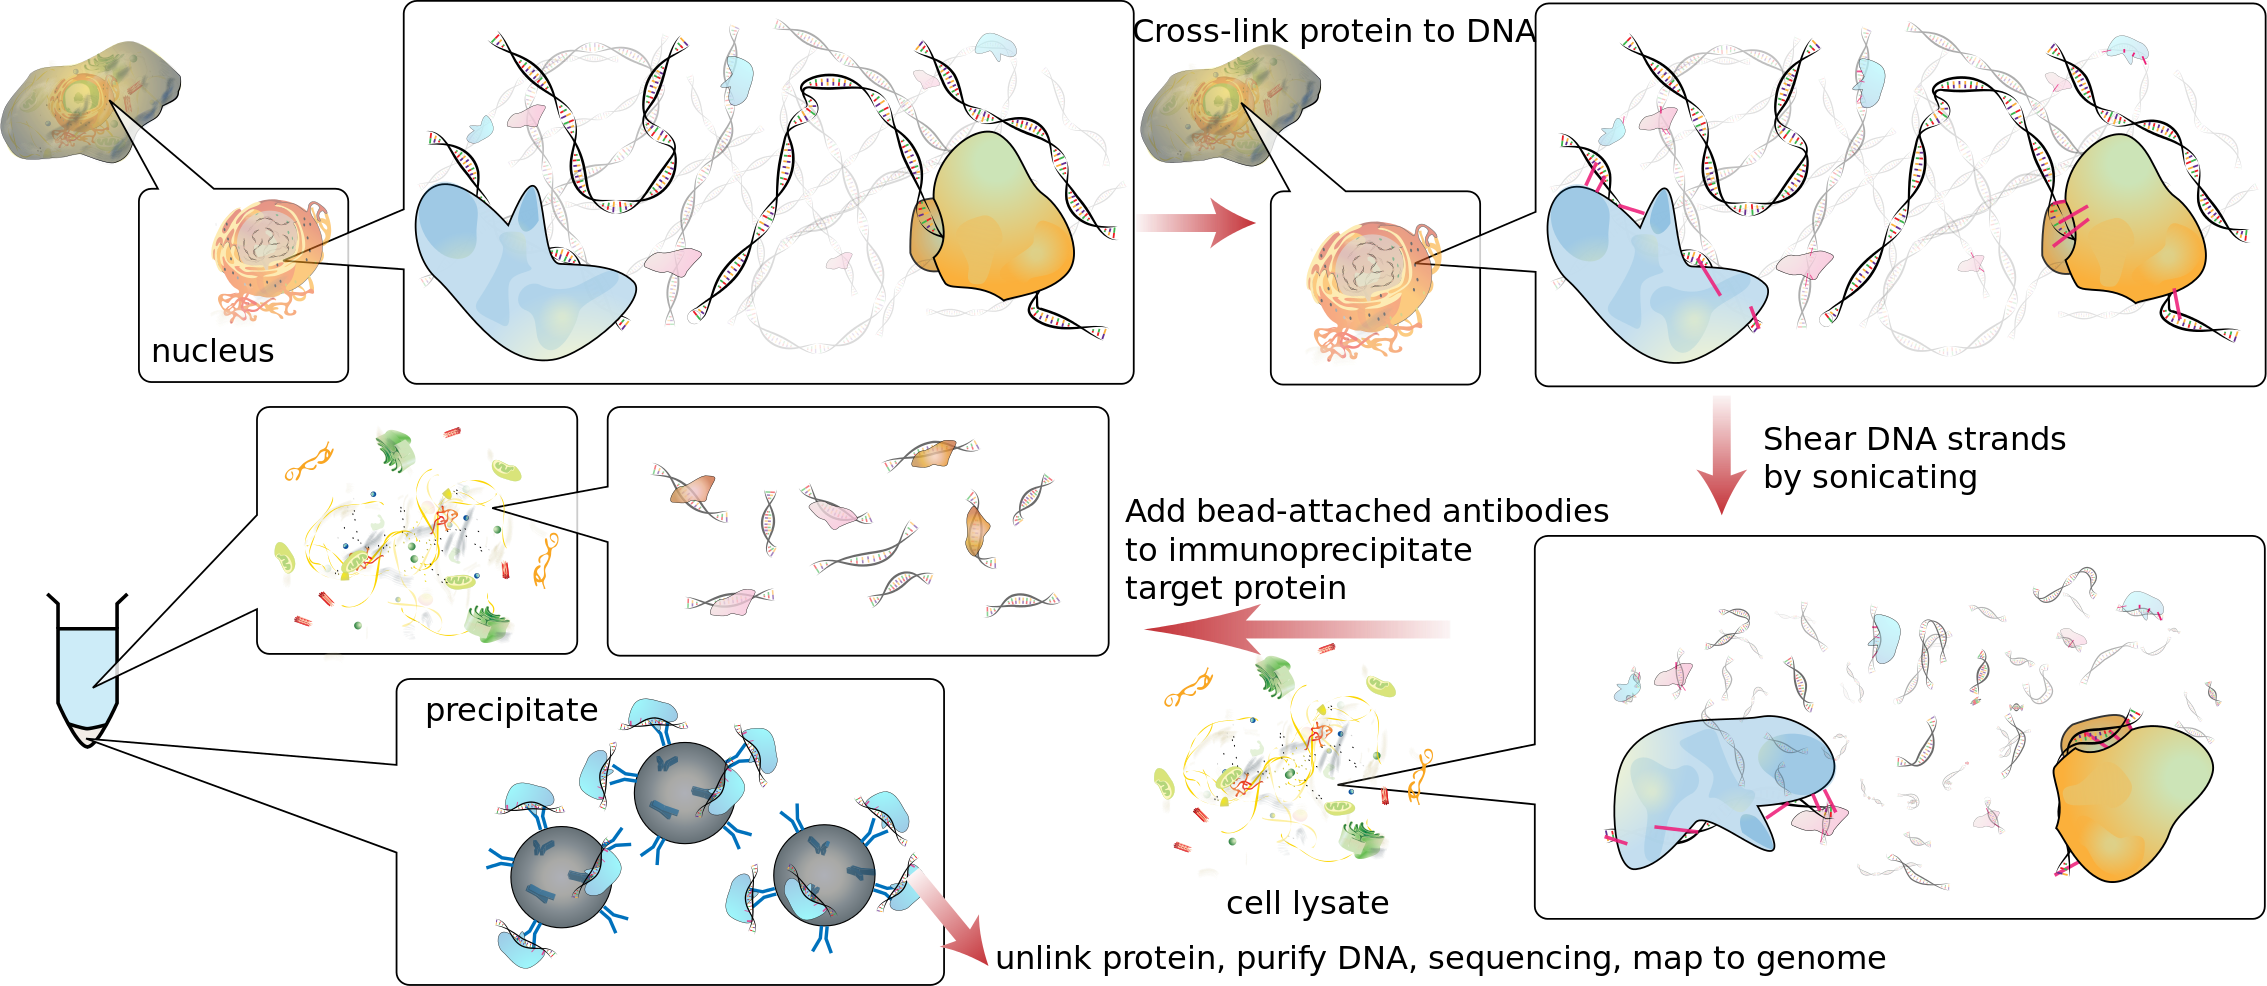
\includegraphics[width=\textwidth]{Chromatin_immunoprecipitation_sequencing_wide.png}

  Source: ``ChIP-sequencing,'' Wikipedia.
\end{frame}

\begin{frame}
  \frametitle{Problem: find peaks in each of several samples}
  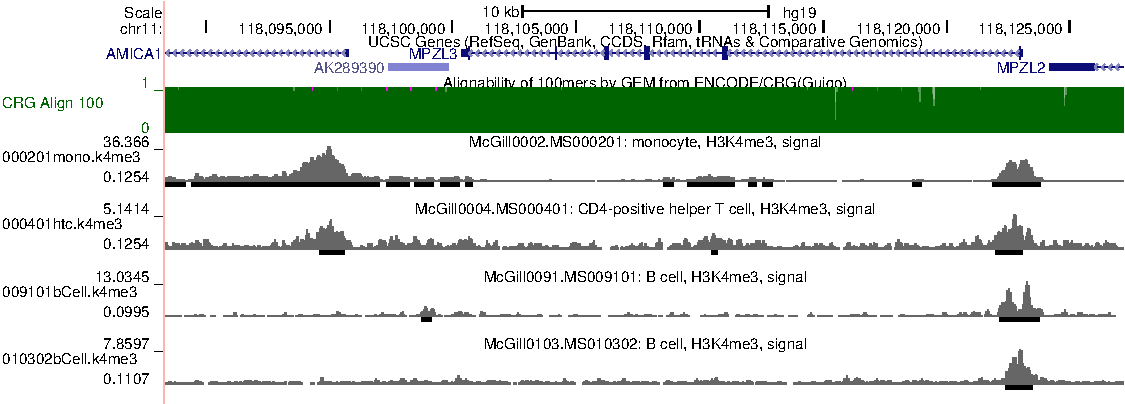
\includegraphics[width=\textwidth]{screenshot-ucsc-edited}

  Grey profiles are normalized aligned read count signals.

  Black bars are ``peaks'' called by MACS2 (Zhang et al, 2008):
  \begin{itemize}
  \item \alert<1>{many false positives}.
  \item overlapping peaks have different start/end positions.
  \end{itemize}
\end{frame}

\begin{frame}
  \frametitle{Previous work in genomic peak detection}
  \begin{itemize}
  \item Model-based analysis of ChIP-Seq (MACS), Zhang et al, 2008.
  \item SICER, Zang et al, 2009.
  \item HOMER, Heinz et al, 2010.
  \item CCAT, Xu et al, 2010.
  \item RSEG, Song et al, 2011.
  \item Triform, Kornacker et al, 2012.
  \item Histone modifications in cancer (HMCan), Ashoor et al, 2013.
  \item PeakSeg, Hocking, Rigaill, Bourque, ICML 2015.
  \item PeakSegJoint Hocking and Bourque, arXiv:1506.01286.
  \item ... dozens of others.
  \end{itemize}
  Two big questions: how to choose the best...
  \begin{itemize}
  \item ...algorithm? (testing)
  \item \alert<1>{...parameters? (training)}
  \end{itemize}
\end{frame}

\begin{frame}[fragile]
  \frametitle{How to choose parameters of unsupervised peak
    detectors?}
\scriptsize
19 parameters for Model-based analysis of ChIP-Seq (MACS), Zhang et al, 2008.
\begin{verbatim}
  [-g GSIZE]
  [-s TSIZE] [--bw BW] [-m MFOLD MFOLD] [--fix-bimodal]
  [--nomodel] [--extsize EXTSIZE | --shiftsize SHIFTSIZE]
  [-q QVALUE | -p PVALUE | -F FOLDENRICHMENT] [--to-large]
  [--down-sample] [--seed SEED] [--nolambda]
  [--slocal SMALLLOCAL] [--llocal LARGELOCAL]
  [--shift-control] [--half-ext] [--broad]
  [--broad-cutoff BROADCUTOFF] [--call-summits]
\end{verbatim}
10 parameters for Histone modifications in cancer (HMCan),
Ashoor et al, 2013.
\begin{verbatim}
minLength 145
medLength 150
maxLength 155
smallBinLength 50
largeBinLength 100000
pvalueThreshold 0.01
mergeDistance 200
iterationThreshold 5
finalThreshold 0
maxIter 20
\end{verbatim}
\end{frame}

\begin{frame}
  \frametitle{Which macs parameter is best for these data?}
  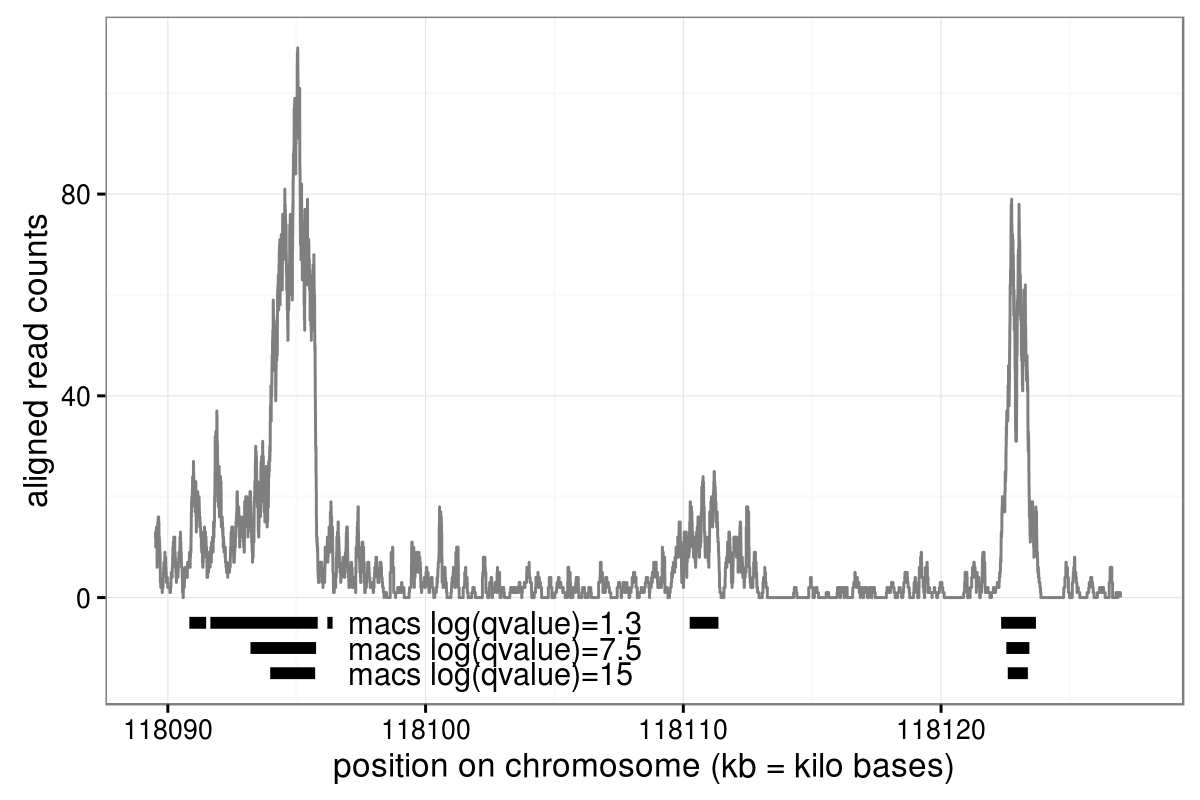
\includegraphics[width=1\textwidth]{figure-macs-problem.png}
\end{frame}

\begin{frame}
  \frametitle{Compute likelihood/loss of piecewise constant model}
  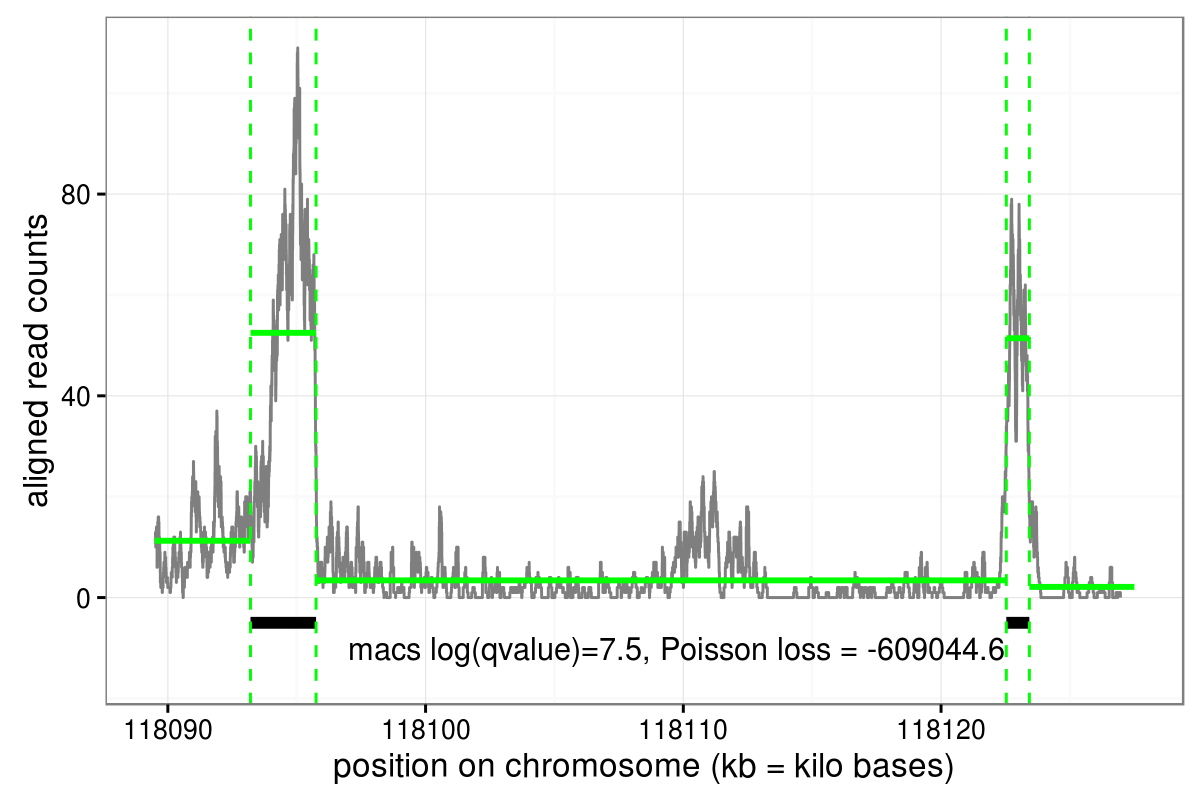
\includegraphics[width=1\textwidth]{figure-macs-problem-7-5.png}
  % $\PoissonLoss(\mathbf z, \mathbf m) = \sum_{i=1}^n m_i - z_i \log(m_i)$
  % for count data $\mathbf z\in\ZZ_+^n$ 
  % and segment mean model $\mathbf m\in\RR^n$.
\end{frame}

\begin{frame}
  \frametitle{Idea: choose the parameter with a lower loss}
  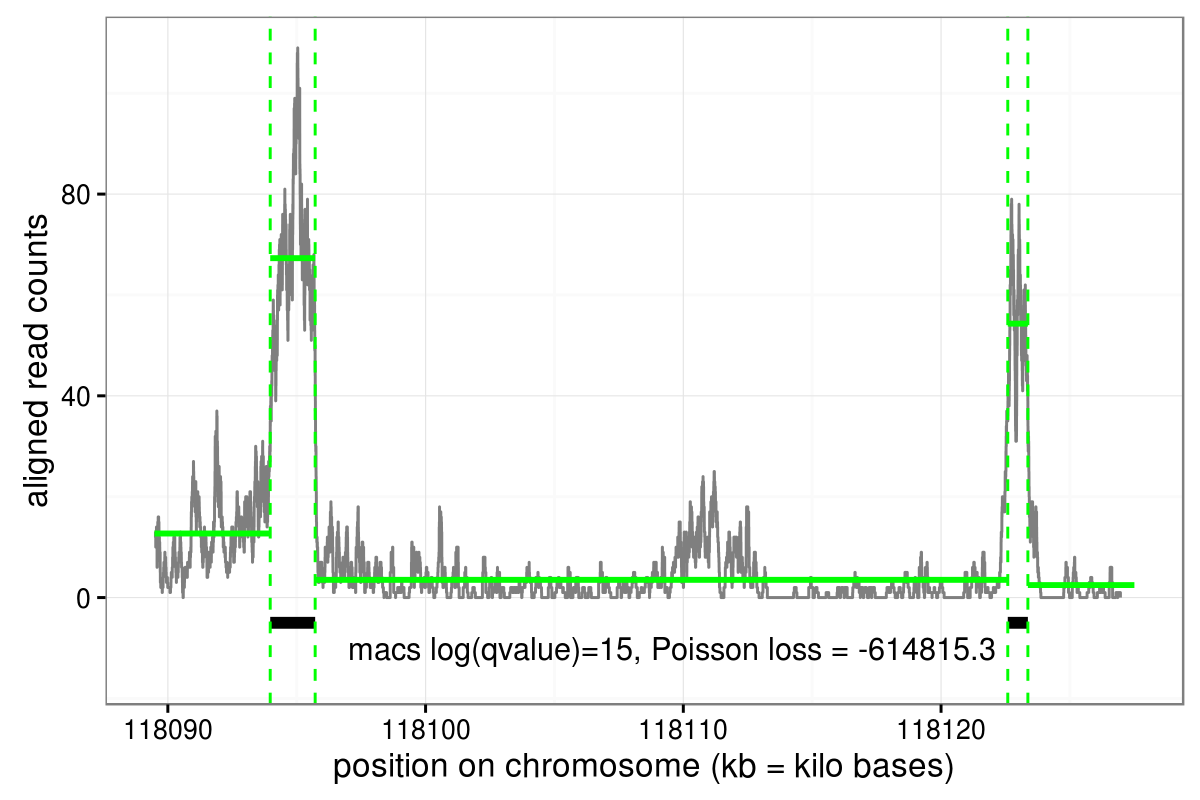
\includegraphics[width=1\textwidth]{figure-macs-problem-15.png}
\end{frame}

\begin{frame}
  \frametitle{PeakSeg: search for the peaks with lowest loss}
  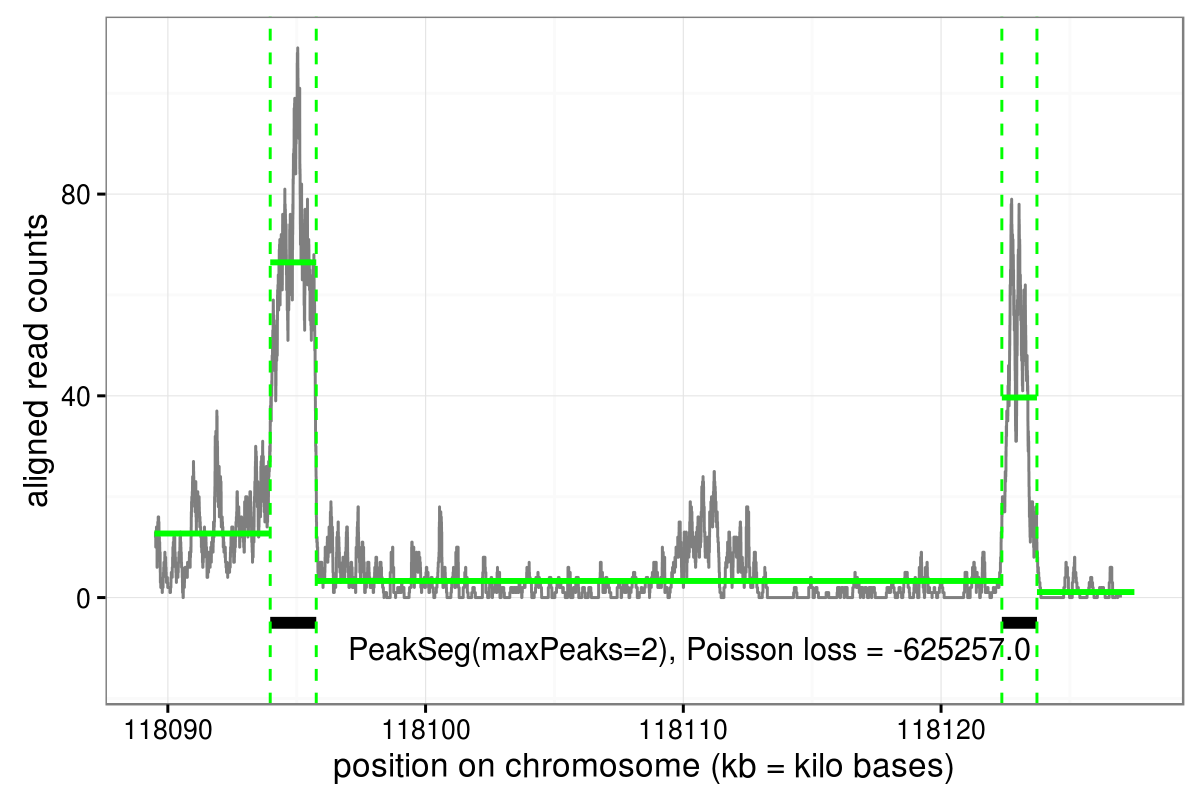
\includegraphics[width=1\textwidth]{figure-macs-problem-PeakSeg.png}

  Choose the number of peaks via standard penalties (AIC, BIC,
    ...)\\or learned penalties based on visual labels (more on this later).
\end{frame}

\begin{frame}
  \frametitle{Maximum likelihood Poisson segmentation models}
  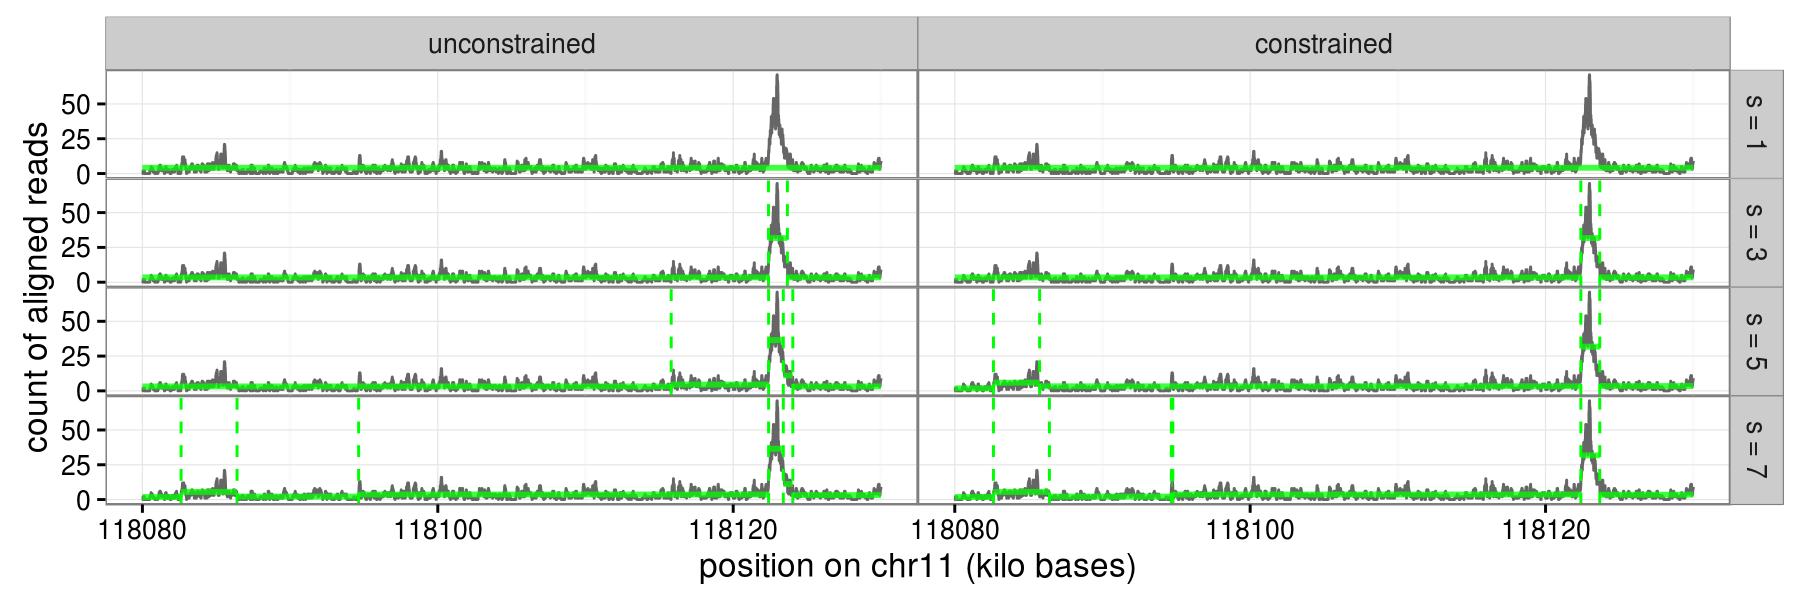
\includegraphics[width=1\textwidth]{figure-Segmentor-PeakSeg}

  \begin{itemize}
  \item Previous work: unconstrained maximum likelihood mean\\
    for $s$ segments ($s-1$ changes), Cleynen et al 2014.
  \item Hocking et al, ICML 2015: PeakSeg constraint enforces up, down, up,
    down changes (and not up, up, down). 
  \item Odd-numbered segments are background noise,\\
    even-numbered segments are peaks.
  \item Constrained Dynamic Programming Algorithm, 
    $O(N^2)$ time for $N$ data points.
  \end{itemize}
\end{frame}

\begin{frame}
  \frametitle{But quadratic time is not fast enough for genomic data!}
  \includegraphics[width=\textwidth]{figure-PDPA-timings-dp}
  \begin{itemize}
  \item Genomic data is large, $N \geq 10^6$.
  \item Split into subsets? What if we split a peak in half?
  \item Need linear time algorithm for analyzing whole data set.
  \end{itemize}
\end{frame}

\section{Segment neighborhood model (constraint on number of peaks)}

\begin{frame}
  \frametitle{Statistical model is Poisson with change constraints}
  \begin{itemize}
  \item We have $N$ count data $z_1, \dots, z_N\in\ZZ_+$.
  \item Fix the number of segments $S\in\{1, 2, \dots, N\}$.
  \item PeakSeg Model: $z_t \sim \text{Poisson}(m_t)$ such that $m_t$
    has $S-1$ up-down changes.
  \item Want to find means $m_t$ which maximize the Poisson likelihood:
    $P(Z = z_t|m_t) = m_t^{z_t} e^{-m_t} / (z_t!)$.
  \item Equivalent to finding means $m_t$ which minimize the Poisson
    loss: $\ell(m_t, z_t) = m_t - z_t\log m_t$.
  \item Naive computation is $O(N^S)$, since there are $O(N^{S-1})$ possible
    positions for $S-1$ change-points, and it takes $O(N)$ operations to
    compute the mean and loss for each.
  \item Comparison to Hidden Markov Model:
    \begin{description}
    \item[Likelihood] Same emission terms, no transition terms.
    \item[Constraint] Number of changes rather than values.
    \end{description}
  \end{itemize}
\end{frame}

\begin{frame}
  \frametitle{Relation to previous dynamic programming algorithms}
  \begin{tabular}{r|c|c}
    & no pruning & functional pruning \\
    \hline
    unconstrained & \alert<1>{Dynamic Programming} & \alert<2>{Pruned DP} \\
     & \alert<1>{exact $O(SN^2)$} & \alert<2>{exact $O(SN\log N)$}\\
    R pkgs: & \alert<1>{changepoint} & \alert<2>{cghseg, Segmentor}\\
    \hline
    up-down constrained & \alert<3>{constrained DP} & \alert<4>{\textbf{this work}} \\
     & \alert<3>{inexact $O(SN^2)$} & \alert<4>{exact $O(SN\log N)$}\\
    R pkgs: & \alert<3>{PeakSegDP} & \alert<4>{coseg}\\
    \hline
  \end{tabular}
  \begin{itemize}
  \item \alert<1>{Auger and Lawrence, Algorithms for the optimal
      identification of segment neighborhoods (Bull Math Biol 1989).}
  \item \alert<2>{Independent discovery: Rigaill 2010, Johnson
      2013. R package Segmentor: Cleynen et al 2014.}
  \item \alert<3>{Hocking, Rigaill, Bourque 2015.}
  \item \alert<4>{\textbf{Contribution}: new algorithm that
      \textbf{exactly} computes the \textbf{constrained} optimal
      segmentation for $N$ data points and $1,\dots,S$ segments in $O(S N\log N)$ time.}
  \end{itemize}
\end{frame}


\begin{frame}
  \frametitle{Dynamic programming and functional pruning}
  \textbf{Classical dynamic programming} (Auger and Lawrence 1989)
  computes the matrix of optimal loss values in $S$ segments up to $N$
  data points, $O(S N^2)$
$$
\begin{array}{ccc}
  \mathcal L_{1,1} & \cdots &   \mathcal L_{1,N}\\
  \vdots &  & \vdots\\
  \mathcal L_{S,1} & \cdots & \mathcal L_{S,N}\\
\end{array}
$$
\textbf{Dynamic programming with functional pruning} (Rigaill 2010,
Johnson 2013) computes a matrix of loss \textbf{functions}, the
optimal loss up to $N$ data points if segment $S$ has mean $\mu_S$,
$O(S N\log N)$
$$
\begin{array}{ccc}
   L_{1,1}(\mu_1) & \cdots & L_{1,N}(\mu_1)\\
  \vdots &  & \vdots\\
   L_{S,1}(\mu_S) & \cdots & L_{S,N}(\mu_S),\\
\end{array}
$$
\textbf{Contribution of this work}: a new algorithm that applies the
functional pruning technique to the up-down constrained model.
\end{frame}

\begin{frame}
  \frametitle{First segment, first data point}
  \begin{itemize}
  \item For data $z_1, \dots, z_N\in\ZZ_+$ let
  \begin{equation*}
    \gamma_t(\mu) = \ell(\mu, z_t) = \mu - z_t \log \mu
  \end{equation*}
  be the Poisson loss for each $t\in\{1, \dots, N\}$.
\item For example $z = 2, 1, 0, 4$.
\item Then $\gamma_1(\mu)=L_{1,1}(\mu)= \alert{1}\mu - \alert{2}\log \mu + \alert{0}$.
\item Need to store 3 coefficients (\alert{linear}, \alert{log}, \alert{constant}).
  \end{itemize}
  \begin{center}
    \includegraphics[width=0.7\textwidth]{figure-PeakSegPDPA-demo-cost-1segments-1data}
  \end{center}
\end{frame}

\begin{frame}
  \frametitle{First segment, other data points}
  \begin{itemize}
\item
  The loss of the first segment up to data point $t$ is
  \begin{equation*}
    \label{eq:C1b}
    L_{1,t}(\mu) = \sum_{i=1}^t \gamma_i(\mu).
  \end{equation*}
\item For example $z = 2, 1, 0, 4$.
% \item $L_{1,2}(\mu) = (2\mu - 3\log\mu + 0)/2 = 1\mu - 1.5\log\mu + 0$.
% \item $L_{1,3}(\mu) = (3\mu - 13\log\mu + 0)/3 = 1\mu - 4.333\log\mu + 0$.
\item $L_{1,2}(\mu) = 2\mu - 3\log\mu + 0$.
\item $L_{1,3}(\mu) = 3\mu - 12\log\mu + 0$.
\item ...
  \end{itemize}
  \begin{center}
    \includegraphics[width=0.5\textwidth]{figure-PeakSegPDPA-demo-cost-1segments-2data}
    \includegraphics[width=0.5\textwidth]{figure-PeakSegPDPA-demo-cost-1segments-3data}
  \end{center}
\end{frame}

\begin{frame}[fragile]
  \frametitle{Second segment, up to data point 2}
  \begin{itemize}
  \item The mean cost in 2 segments up to data point 2 is
\begin{eqnarray*}
  L_{2,2}(\mu_2) 
  &=&  \gamma_2(\mu_2)+\min_{\mu_1 \leq \mu_2} L_{1,1}(\mu_1)\\
  &=& \gamma_2(\mu_2)+L_{1,1}^{\leq}(\mu_2)
\end{eqnarray*}
\item Min-less operator is $L^\leq(\mu) = \min_{x\leq\mu} L(x),$
    \begin{center}
      \includegraphics[width=0.5\textwidth]{figure-PeakSegPDPA-demo-minlessmore-2segments-2data}
    \end{center}
\end{itemize}
\end{frame}

\begin{frame}
  \frametitle{Comparison with unconstrained Pruned DPA}
  \begin{itemize}
  \item For our constrained algorithm, the first segment mean must be
    less than the second, and the first segment cost is a function:
    \begin{equation*}
      L_{2,2}(\mu_2) = \gamma_2(\mu_2)+
      \underbrace{\min_{\mu_1 \leq \mu_2} L_{1,1}(\mu_1)}_{L^\leq_{1,1}(\mu_2)}.
    \end{equation*}
  \item For the unconstrained algorithm, it is \alert<1>{constant}:
    \begin{equation*}
      \widehat{L}_{2,2}(\mu_2) = \gamma_2(\mu_2)+
      \alert<1>{\underbrace{\min_{\mu_1} L_{1,1}(\mu_1)}_{\mathcal L_{1,1}}}.
    \end{equation*}
  \item For example $z = 2, 1, 0, 4$.
    \begin{center}
      \includegraphics[width=0.5\textwidth]{figure-PeakSegPDPA-demo-mincompare-2segments-2data}
    \end{center}
  \end{itemize}
\end{frame}

\begin{frame}
  \frametitle{Storage as a piecewise function on intervals}
  \begin{itemize}
  \item For example $z = 2, 1, 0, 4$.
    \begin{center}
      \includegraphics[width=0.5\textwidth]{figure-PeakSegPDPA-demo-minlessmore-2segments-2data}
    \end{center}
  \item Storage: 
    \begin{equation*}
      L_{2,2}(\mu) = \gamma_2(\mu) + 
      \begin{cases}
        L_{1,1}(\mu) = 1\mu - 2\log \mu + 0 & \text{ if } \mu\in[0, 2],\\
        \mathcal L_{1,1} = 0\mu -0\log\mu + 0.6137 & \text{ if } \mu\in[2, 4].
      \end{cases}
    \end{equation*}
  \end{itemize}
\end{frame}

 
\begin{frame}[fragile]
  \frametitle{Second segment, up to data point 3}
  \begin{itemize}
  \item For data point 3 we need to consider two change-points:
    \begin{equation*}
      L_{2,3}(\mu) =  \gamma_3(\mu) + \min
      \begin{cases}
        L_{1,2}^{\leq}(\mu), & \text{ change up after data point 2},\\
        L_{2,2}(\mu), & \text{ change up after data point 1}. 
      \end{cases}
    \end{equation*}
  \item For $z = 2, 1, 0, 4$ the min operation prunes a
    change after data point 1.
    \begin{center}
      \includegraphics[width=0.5\textwidth]{figure-PeakSegPDPA-demo-minenv-2segments-3data}
    \end{center}
  \end{itemize}
\end{frame}

\begin{frame}
  \frametitle{Second segment, up to data point t}
  \begin{itemize}
  \item The updates continue for every data point $t\in\{3, ..., N\}$
    \begin{equation*}
      L_{2,t}(\mu) =  \gamma_t(\mu) + \min
      \begin{cases}
        L_{1,t-1}^{\leq}(\mu), & \text{change up after $t-1$,}\\
        L_{2,t-1}(\mu), & \text{change up before $t-1$.}
      \end{cases}
    \end{equation*}
  \item For example for $z = 2, 1, 0, 4$, at data point $t=4$
    we only need to consider changes after 2 and 3 (1 has been
    pruned).
    \begin{center}
      \includegraphics[width=0.5\textwidth]{figure-PeakSegPDPA-demo-minenv-2segments-4data}
    \end{center}
  \end{itemize}
\end{frame}

\begin{frame}
  \frametitle{Dynamic programming for segment neighborhood model}
  \begin{itemize}
  \item Dynamic programming update rule: the constrained cost of a
    mean $\mu$ for the segment $s$, up to data point $t$:
    \begin{equation*}
      L_{s,t}(\mu) = \gamma_t(\mu) + \min
      \begin{cases}
        L_{s,t-1}(\mu),\\
        L_{s-1,t-1}^{*}(\mu),
      \end{cases}
    \end{equation*}
  \item Time complexity of min and min-less/more * is linear in the
    number of intervals, empirically sub-linear $O(\log N)$.
    \includegraphics[width=0.5\textwidth]{figure-PDPA-intervals-all}
  \item Total time complexity: $O(S N\log N)$.
  \end{itemize}
\end{frame}

\section{Results on benchmark data (labeled chromosome subsets)}

\begin{frame}
  \frametitle{Previous work in computer vision: look and add labels
    to...}
  \begin{tabular}{ccc}
    Photos & Cell images & Copy number profiles \\
    \includegraphics[width=1.3in]{../chip-seq-paper/faces} &
    \includegraphics[width=1.3in]{../chip-seq-paper/cellprofiler} &
    \includegraphics[width=1.5in]{../chip-seq-paper/regions-axes}\\
    Labels: names & phenotypes & alterations \\ \\
    CVPR 2013 & CellProfiler & SegAnnDB \\
    246 papers & 873 citations & Hocking et al, 2014. \\
     &
  \end{tabular}
  Sources: \url{http://en.wikipedia.org/wiki/Face_detection}\\
  Jones et al PNAS 2009. Scoring diverse cellular morphologies in
  image-based screens with iterative feedback and machine learning.
\end{frame}

\begin{frame}
  \frametitle{Benchmark data sets, algorithms}

 \url{http://cbio.ensmp.fr/~thocking/chip-seq-chunk-db/}
  \begin{itemize}
  \item Hocking \emph{et al} Bioinformatics (2016). Optimizing
    ChIP-seq peak detectors using visual labels and supervised machine
    learning.
  \item 37 labeled H3K4me3 samples (sharp peak pattern).
  \item 29 labeled H3K36me3 samples (broad peak pattern).
  \item 12,826 labeled regions with and without peaks.
  \item 2,752 separate segmentation problems.
  \end{itemize}

  Algorithms for segmenting $N$ data points:
  \begin{center}
  \begin{tabular}{ccccc}
    package & constraint & exact? & complexity \\
    \hline
    \textbf{coseg (this work)} & $\mu_1 \leq \mu_2 \geq \mu_3 \dots$ & yes & $O(N\log N)$ \\
    PeakSegDP & $\mu_1 < \mu_2 > \mu_3 \dots$ & no & $O(N^2)$\\
    Segmentor & none & yes & $O(N\log N)$
  \end{tabular}

  \vskip 0.5cm

  Segmentor loss $\leq$ coseg loss $\leq$ PeakSegDP loss.
  \end{center}
\end{frame}

\begin{frame}
  \frametitle{Linear time algorithms faster for larger data sets}
  \includegraphics[width=1\textwidth]{figure-PDPA-timings.pdf}

  Total time to compute 10 models (0, ..., 9 peaks) for all data sets:
  \begin{itemize}
  \item PeakSegDP: 156 hours, inexact.
  \item coseg: 6 hours, exact.
  \end{itemize}
\end{frame}

\begin{frame}
  \frametitle{8 false negative labels for models with 0 peaks}
  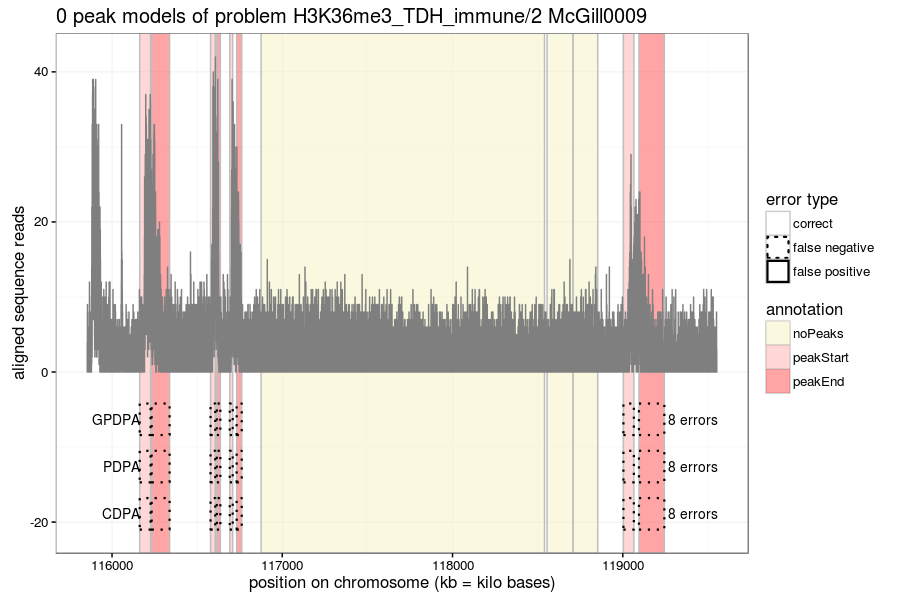
\includegraphics[width=\textwidth]{figure-min-train-error-problem5-0peaks}
\end{frame}

\begin{frame}
  \frametitle{Models with 1 peak are better (6 FN)}
  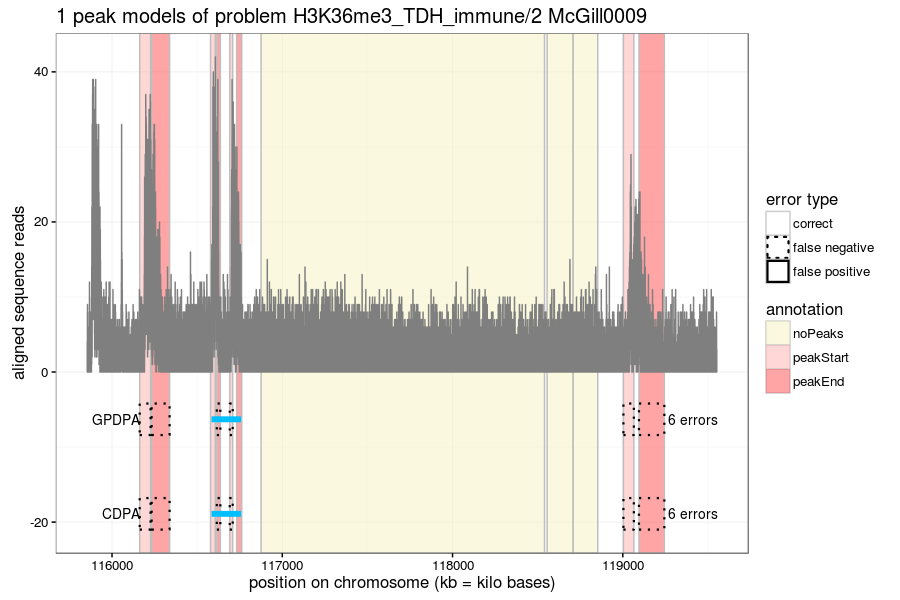
\includegraphics[width=\textwidth]{figure-min-train-error-problem5-1peaks}
\end{frame}

\begin{frame}
  \frametitle{Models with 2 peaks are better still (4 FN)}
  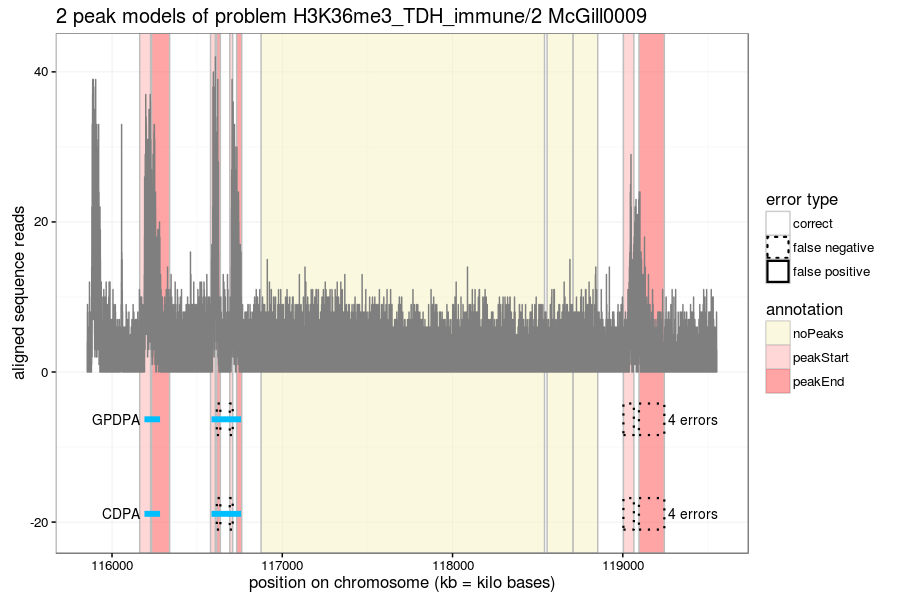
\includegraphics[width=\textwidth]{figure-min-train-error-problem5-2peaks}
\end{frame}

\begin{frame}
  \frametitle{Models with 3 peaks are the same (4 FN)}
  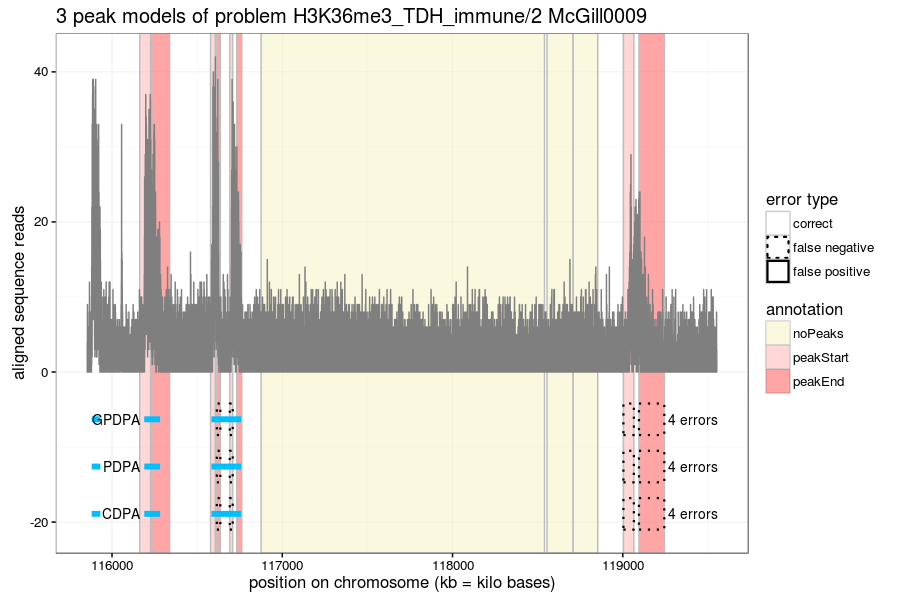
\includegraphics[width=\textwidth]{figure-min-train-error-problem5-3peaks}
\end{frame}

\begin{frame}
  \frametitle{Models with 4 peaks are better (2 FN)}
  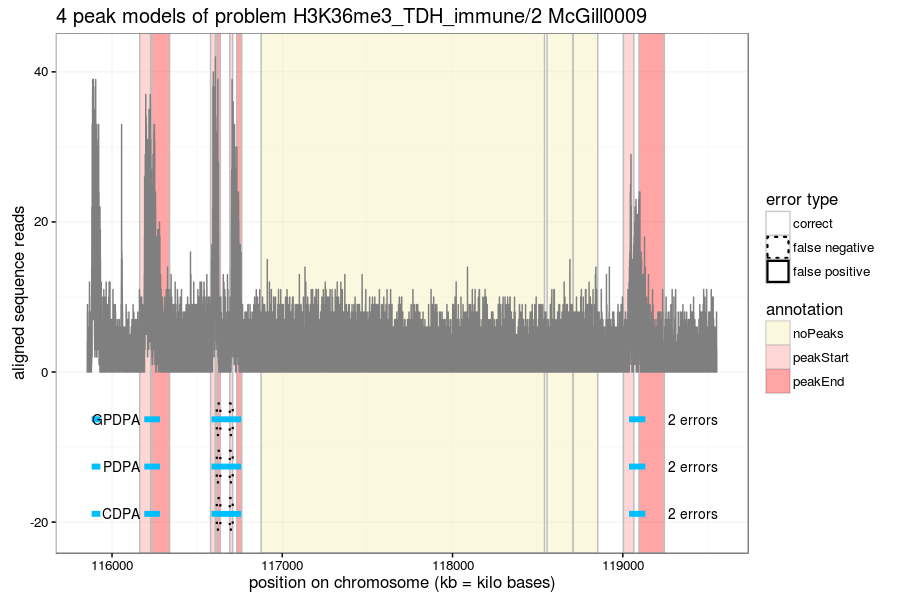
\includegraphics[width=\textwidth]{figure-min-train-error-problem5-4peaks}
\end{frame}

\begin{frame}
  \frametitle{Models with 5 peaks have no incorrect labels}
  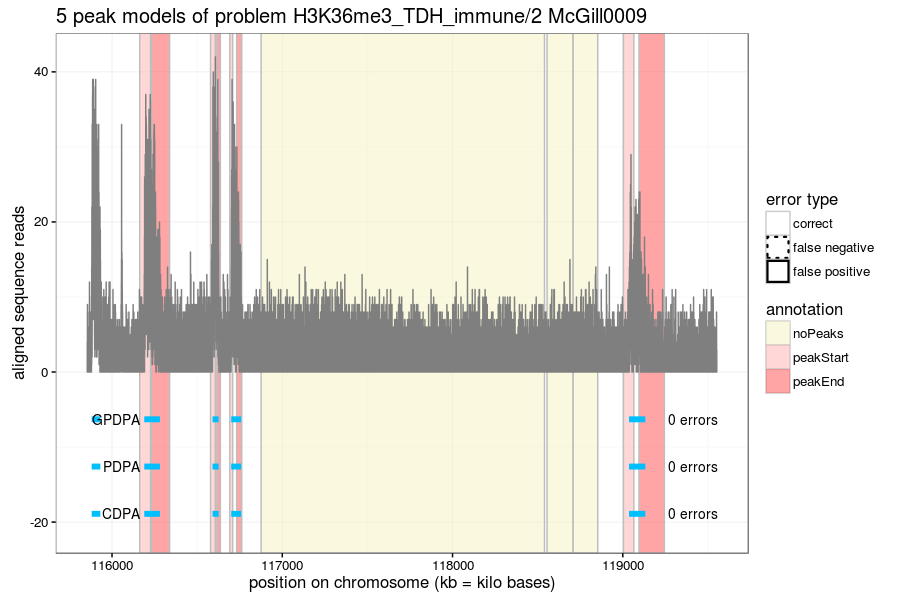
\includegraphics[width=\textwidth]{figure-min-train-error-problem5-5peaks}
\end{frame}


\begin{frame}
  \frametitle{Models with 6 peaks are worse (1 false positive)}
  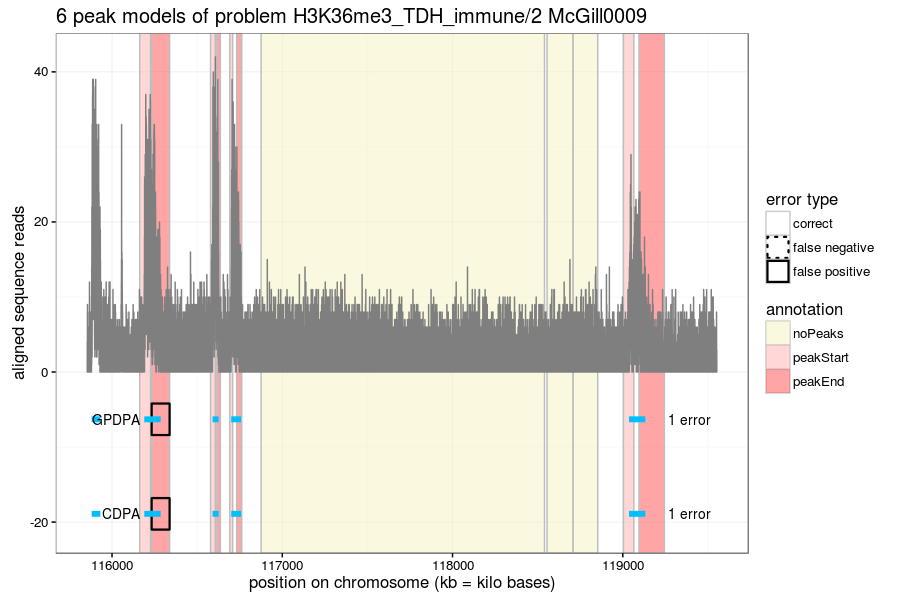
\includegraphics[width=\textwidth]{figure-min-train-error-problem5-6peaks}
\end{frame}

\begin{frame}
  \frametitle{Constrained optimization better than macs}
  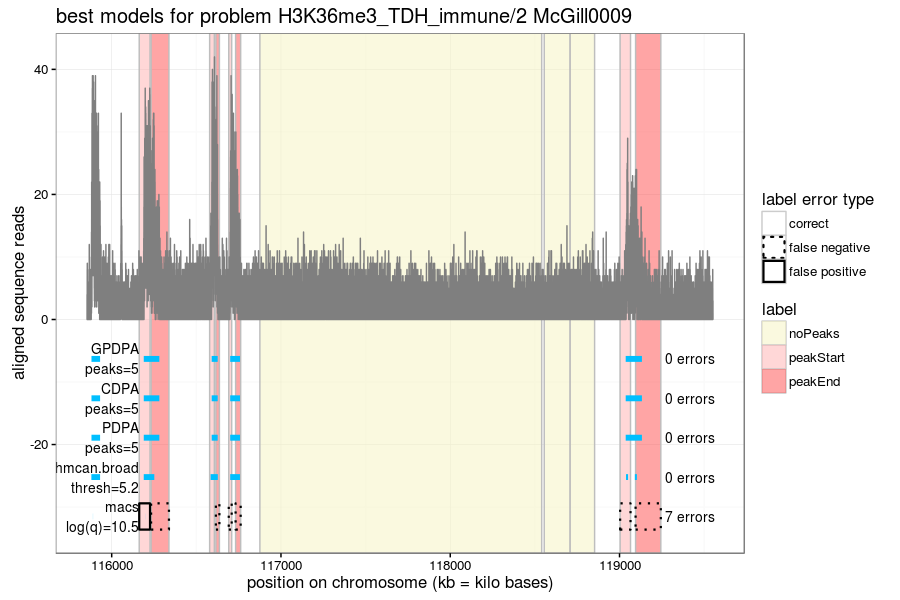
\includegraphics[width=\textwidth]{figure-min-train-error-problem5-best}
\end{frame}

\begin{frame}
  \frametitle{0 errors for coseg/PeakSegDP, 6 errors for Segmentor}
  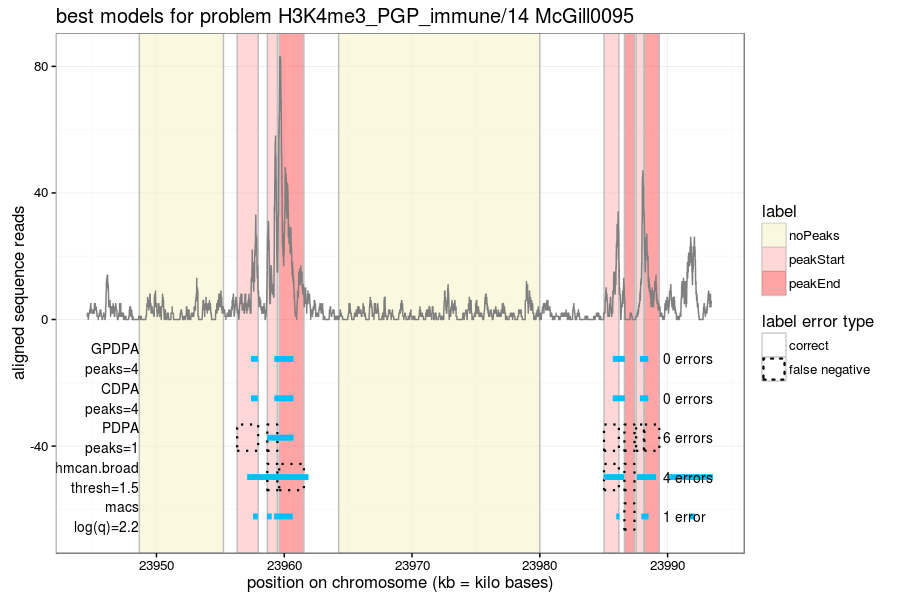
\includegraphics[width=\textwidth]{figure-min-train-error-problem2-best.png}
\end{frame}


% \begin{frame}
%   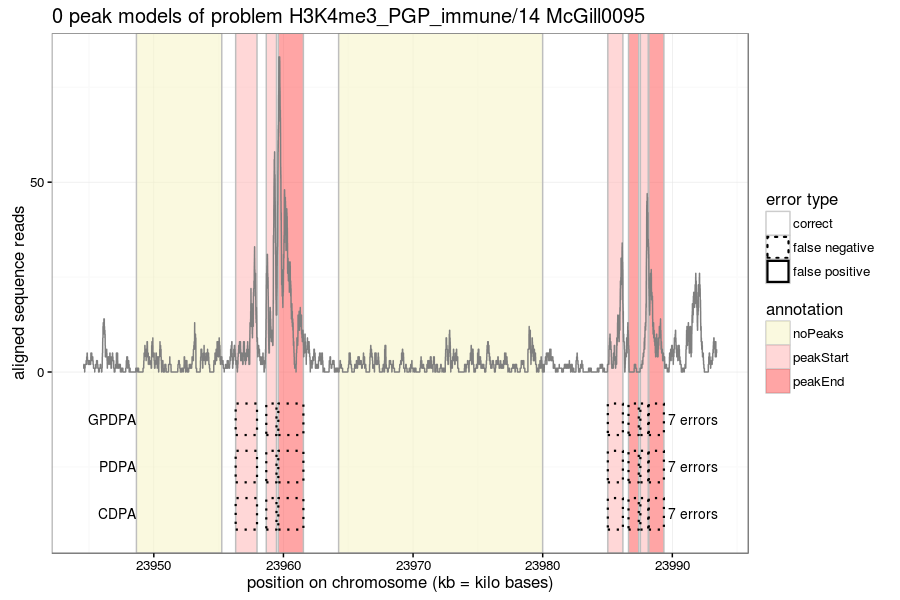
\includegraphics[width=\textwidth]{figure-min-train-error-problem2-0peaks.png}
% \end{frame}

% \begin{frame}
%   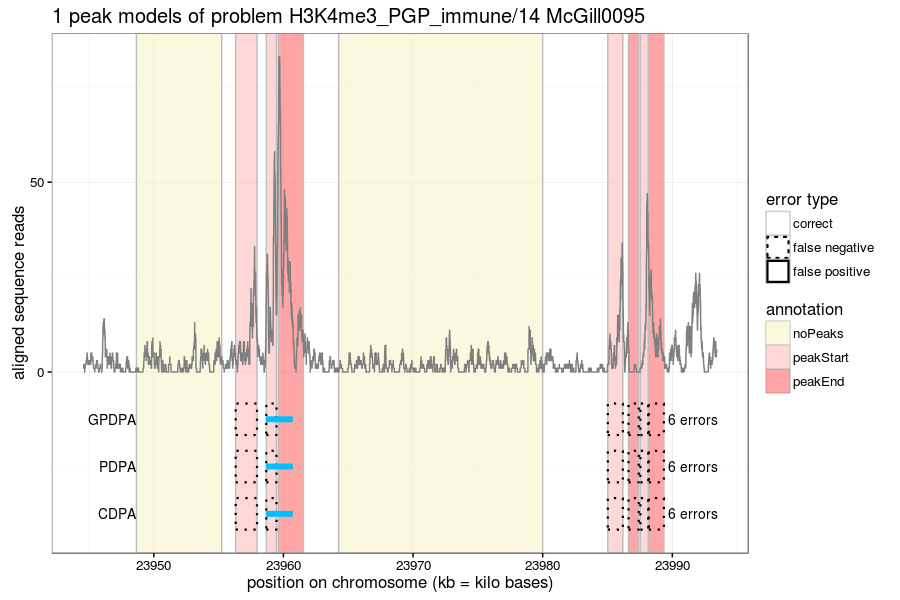
\includegraphics[width=\textwidth]{figure-min-train-error-problem2-1peaks.png}
% \end{frame}

% \begin{frame}
%   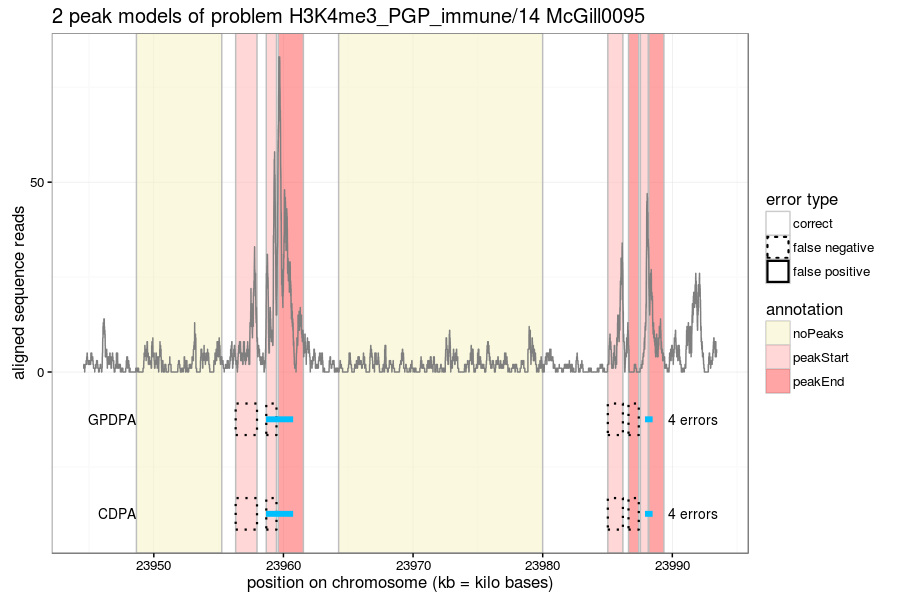
\includegraphics[width=\textwidth]{figure-min-train-error-problem2-2peaks.png}
% \end{frame}

% \begin{frame}
%   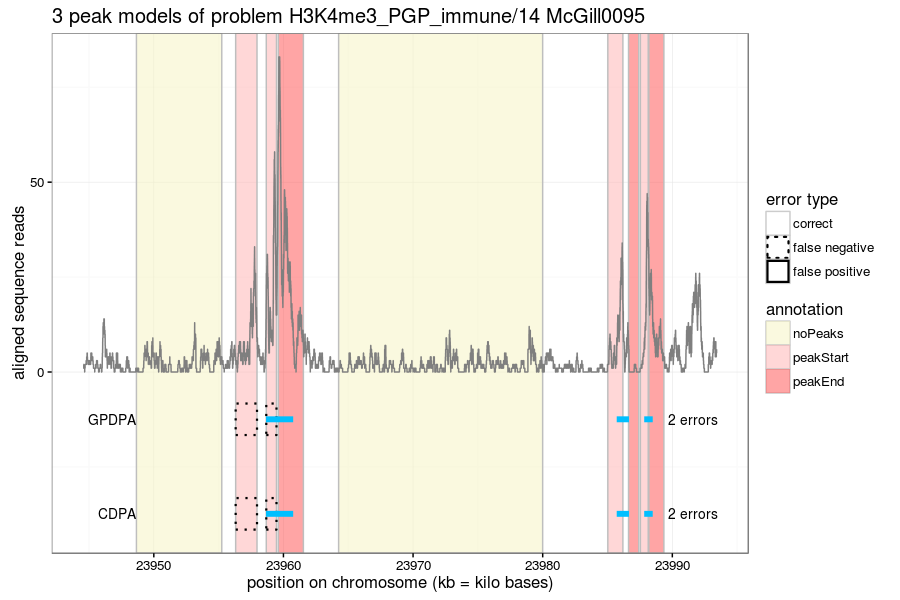
\includegraphics[width=\textwidth]{figure-min-train-error-problem2-3peaks.png}
% \end{frame}

% \begin{frame}
%   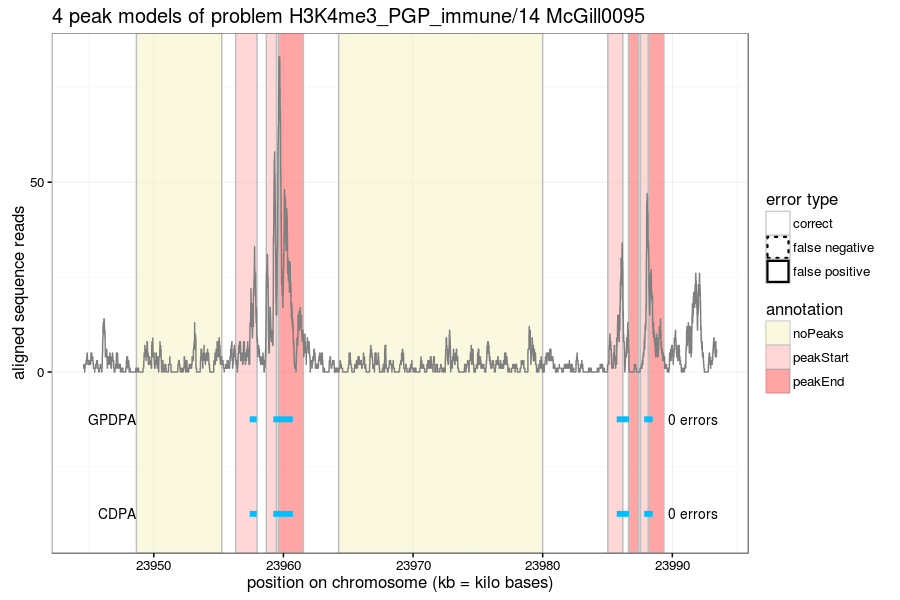
\includegraphics[width=\textwidth]{figure-min-train-error-problem2-4peaks.png}
% \end{frame}

% \begin{frame}
%   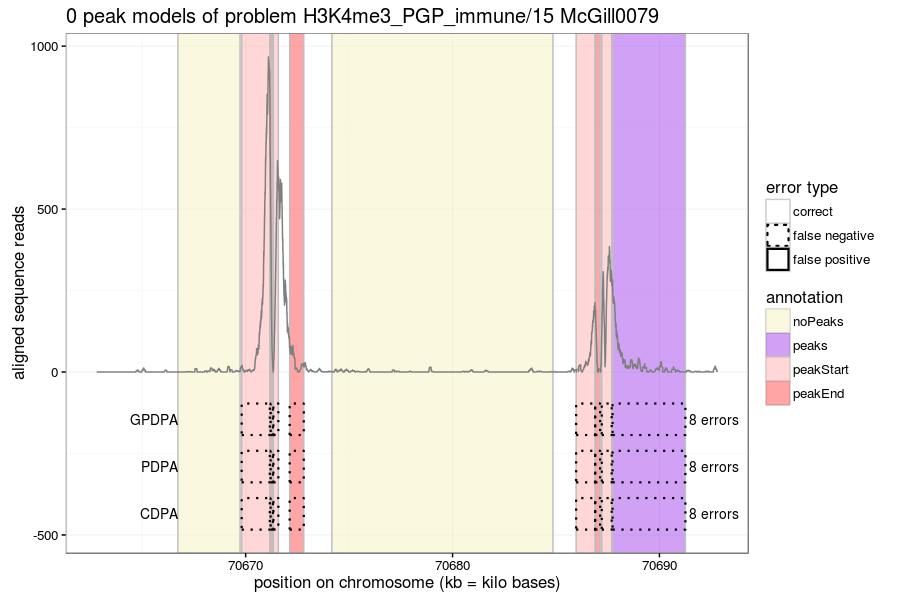
\includegraphics[width=\textwidth]{figure-min-train-error-problem1-0peaks.png}
% \end{frame}

% \begin{frame}
%   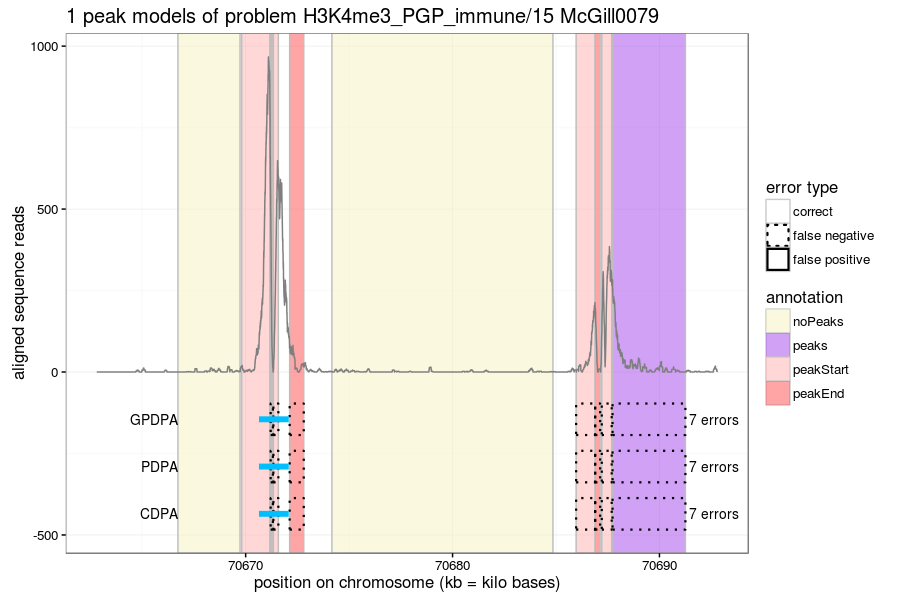
\includegraphics[width=\textwidth]{figure-min-train-error-problem1-1peaks.png}
% \end{frame}

% \begin{frame}
%   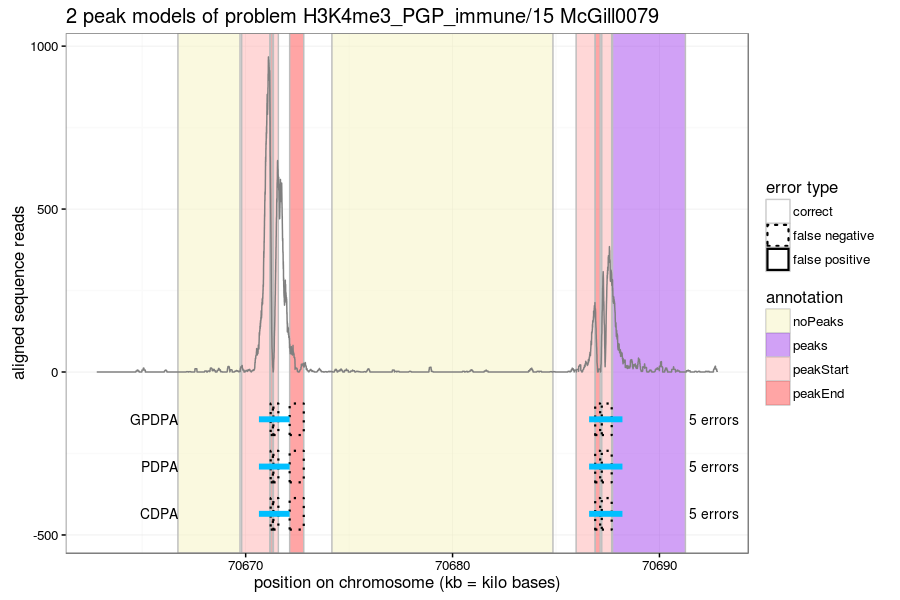
\includegraphics[width=\textwidth]{figure-min-train-error-problem1-2peaks.png}
% \end{frame}

% \begin{frame}
%   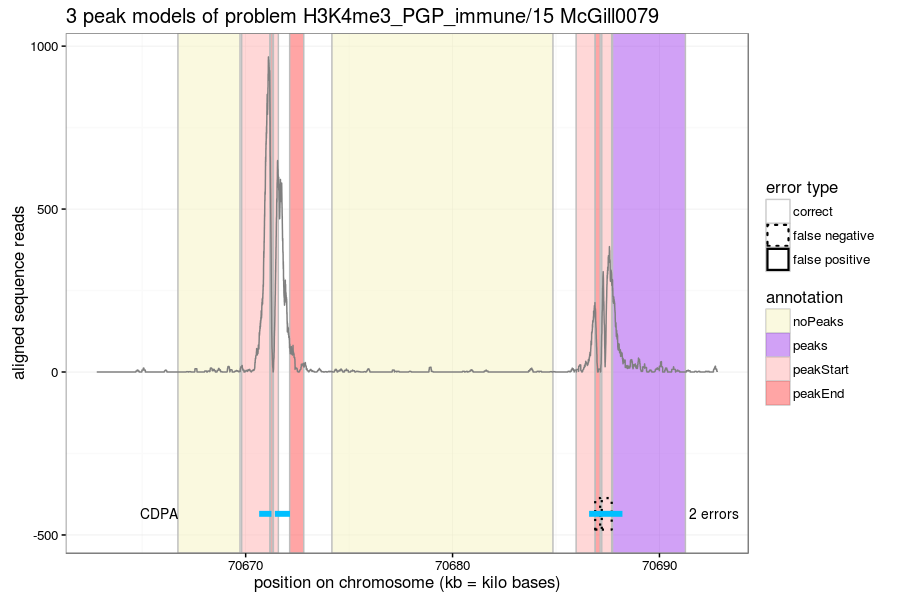
\includegraphics[width=\textwidth]{figure-min-train-error-problem1-3peaks.png}
% \end{frame}

% \begin{frame}
%   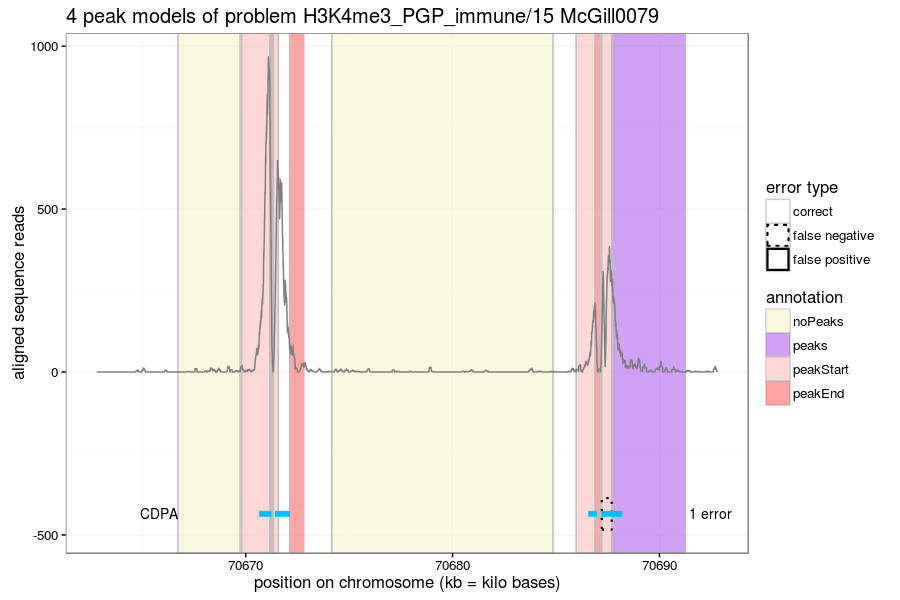
\includegraphics[width=\textwidth]{figure-min-train-error-problem1-4peaks.png}
% \end{frame}

\begin{frame}
  \frametitle{Minimum train error in all data sets}
  \begin{center}
      % latex table generated in R 3.3.3 by xtable 1.7-4 package
% Wed Jun 21 17:03:48 2017
\begin{tabular}{rrrrr}
  \hline
 & errors & fp & fn & feasible models \\ 
  \hline
CDPA & 677 & 116 & 561 & 27469 \\ 
  GPDPA & 789 & 94 & 695 & 21278 \\ 
  macs & 1293 & 519 & 774 &  \\ 
  PDPA & 1544 & 46 & 1498 & 8106 \\ 
  hmcan.broad & 2778 & 367 & 2411 &  \\ 
  \hline possible & 12826 & 11037 & 7225 & 27520 \\ 
   \hline
\end{tabular}

  \end{center}
  \begin{itemize}
  \item Segmentor, PeakSegDP, coseg were used to compute up to 10
    models for each problem (1,...,19 segments = 0,...,9 peaks).
  \item errors = fp + fn = total number of incorrect labels, after
    picking best parameter for each of the 2752 separate problems.
  \item models = number that obey the up-down constraint.
  \item New coseg algorithm has minimum train error almost as good as
    slower PeakSegDP algorithm.
  \item Other algorithms much less accurate.
  \end{itemize}
\end{frame}

\begin{frame}
  \frametitle{Max-margin penalty learning algortihm}
  \includegraphics[width=\textwidth]{figure-large-margin}

\scriptsize \url{http://bl.ocks.org/tdhock/raw/9311ca39d643d127e04a088814c81ee1/}

\end{frame}

\begin{frame}
  \frametitle{ROC curves for one test fold}
  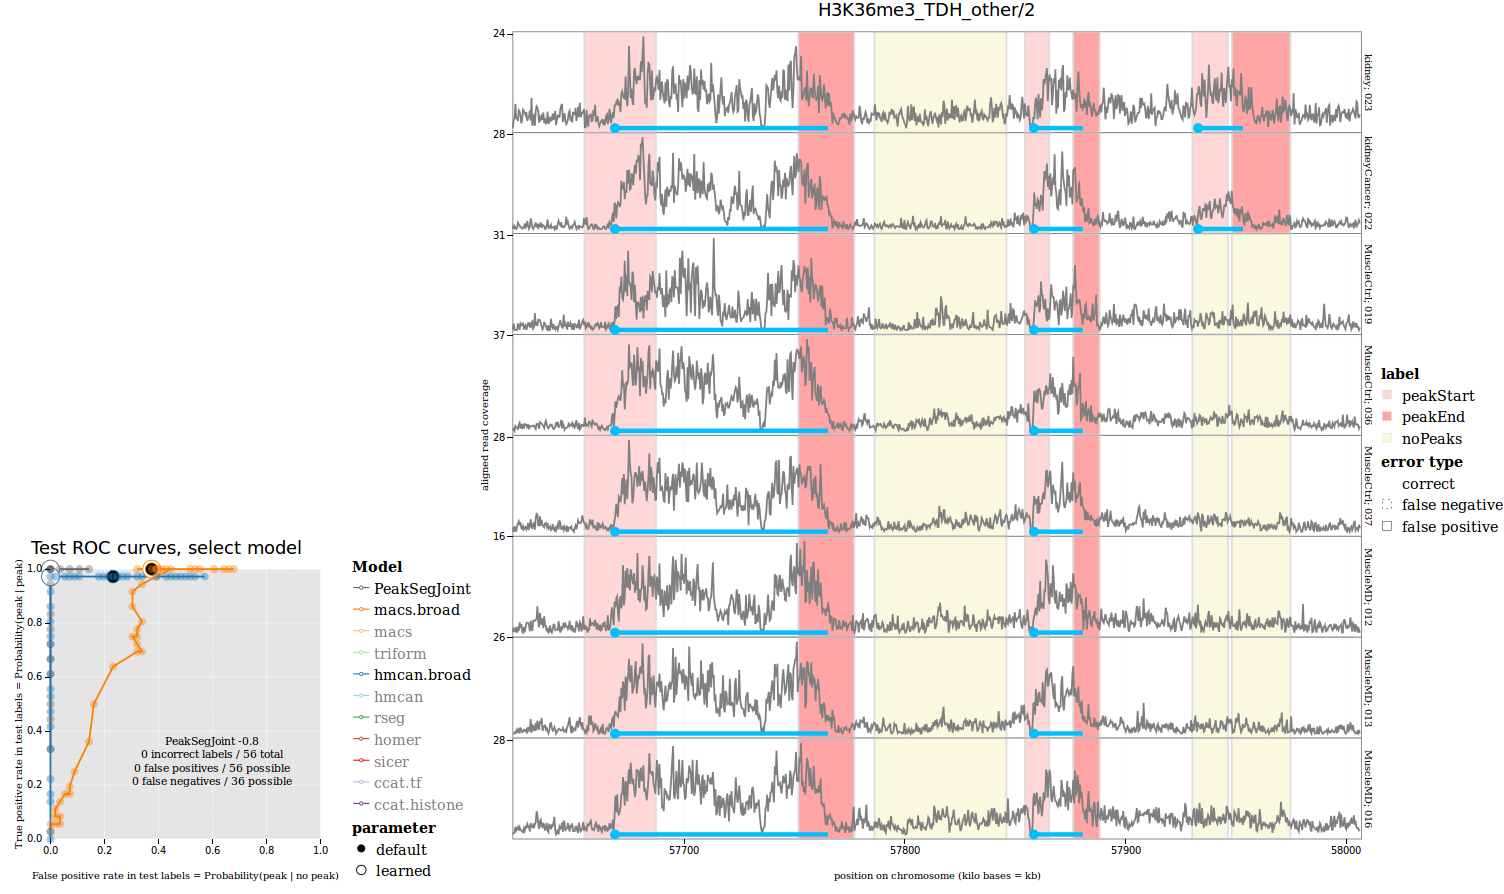
\includegraphics[width=\textwidth]{screenshot-roc-test-interactive}
  
  \scriptsize \url{http://cbio.ensmp.fr/~thocking/chip-seq-chunk-db/figure-roc-test/}
\end{frame}


\begin{frame}
  \frametitle{Test AUC on 7 benchmark data sets}
  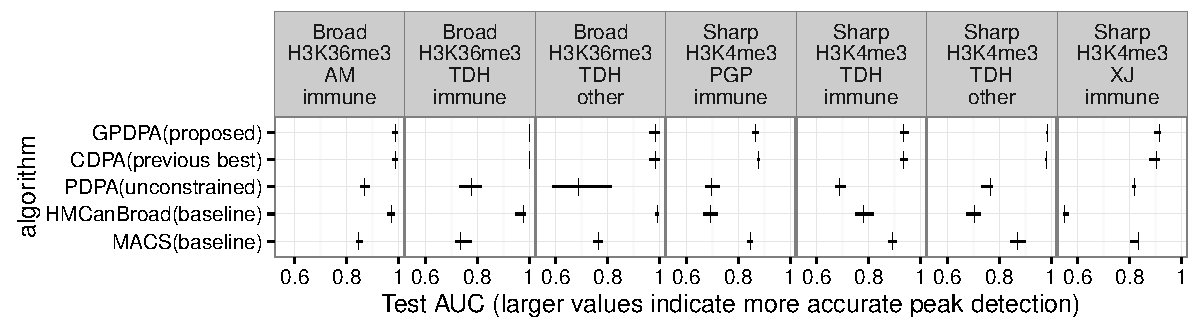
\includegraphics[width=\textwidth]{figure-test-error-dots}
  \begin{itemize}
  \item 4-fold cross-validation: train on 3/4 of labels, test on 1/4.
  \item HMCanBroad is accurate for broad H3K36me3 data but not sharp H3K4me3 data.
  \item MACS is accurate for sharp H3K4me3 but not broad H3K36me3 data.
  \item Unconstrained Segmentor algorithm not as accurate as up-down
    constrained algorithms (coseg, PeakSegDP).
  \item Proposed algorithm in coseg R package yields state-of-the-art
    accuracy in all benchmark data sets.
  \end{itemize}
  \scriptsize
\url{http://bl.ocks.org/tdhock/raw/886575874144c3b172ce6b7d7d770b9f/}
\end{frame}

\begin{frame}
  \frametitle{Segmenting whole chromosomes?}
  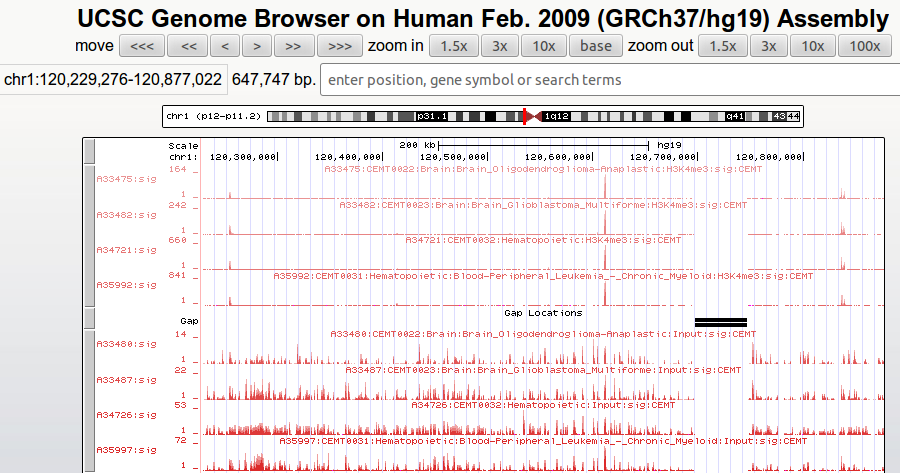
\includegraphics[width=\textwidth]{screenshot-gap-peaks}
  \begin{itemize}
  \item 365 regions with no gaps in hg19.
  \item 272 regions with no gaps on chr1-22, X, Y.
  \item Smallest: 31,833 bases (chr6:157,609,467-157,641,300).
  \item Largest: 115,591,997 bases (chr4:75,452,279-191,044,276).
  \end{itemize}
\end{frame}

\begin{frame}
  \frametitle{But the segment neighborhood algorithm is too slow for
    large genomic regions}
  \begin{itemize}
  \item Time complexity $O(P N \log N)$ to compute models with
    $0,\dots,P$ peaks in $N$ data.
  \item Since $P=O(N)$, time complexity is $O(N^2 \log N)$ -- too slow
    for large genome regions.
  \end{itemize}
  \includegraphics[width=\textwidth]{figure-hg19-problems}
\end{frame}

\section{Optimal partitioning model (penalize number of peaks)}

\begin{frame}
  \frametitle{Optimal partitioning model penalizes the number of changes}
  \begin{itemize}
  \item We have $N$ count data $z_1, \dots, z_N\in\ZZ_+$.
  \item PeakSeg Segment Neighborhood Model: find means $m_t$ which
    minimize the Poisson loss $\sum_{t=1}^N \ell(m_t, z_t)$,
    such that there are exactly $S-1$ up-down changes.
  \item PeakSeg Optimal Partitioning Model: find means $m_t$ with
    up-down changes which minimize the \alert<1>{penalized} Poisson
    loss
    $$\alert<1>{\lambda\sum_{t=1}^{N-1}I(m_t\neq m_{t+1})} + \sum_{t=1}^N \ell(m_t, z_t).$$
  \item No constraint on the number of changes, but $\lambda > 0$
    penalizes models with more changes.
  \end{itemize}
\end{frame}


\begin{frame}
  \frametitle{Relation to previous dynamic programming algorithms}
  \begin{tabular}{r|c|c}
    & no pruning & functional pruning \\
    \hline
    unconstrained & \alert<1>{Dynamic Programming} & \alert<2>{FPOP} \\
     & \alert<1>{exact $O(N^2)$} & \alert<2>{exact $O(N\log N)$}\\
    R packages: &  & \alert<2>{fpop}\\
    \hline
    up-down constrained &  & \alert<3>{\textbf{this work}} \\
     &  & \alert<3>{exact $O(N\log N)$}\\
    R packages: &  & \alert<3>{coseg}\\
    \hline
  \end{tabular}
  \begin{itemize}
  \item \alert<1>{Jackson et al 2005, An algorithm for optimal partitioning of data on an interval.}
  \item \alert<2>{Independent discovery: Johnson 2013, Maidstone et
      al 2016 (FPOP = Functional Pruning Optimal Partitioning).}
  \item \alert<3>{\textbf{Contribution}: new dynamic programming
      algorithm that \textbf{exactly} computes the
      \textbf{constrained} optimal segmentation for $N$ data points
      and a single penalty $\lambda$ in $O(N\log N)$ time.}
  \end{itemize}
  All algorithms compute a model with $S$ segments without having to
  compute models with $1, \dots, S-1$ segments.
\end{frame}

\begin{frame}
  \frametitle{Dynamic programming and functional pruning for the
    optimal partitioning model}
  \textbf{Classical dynamic programming} (Jackson et al 2005) 
  computes the optimal loss values up to $N$ data points, $O(N^2)$
$$
\begin{array}{ccc}
  \mathcal L_{1} & \cdots &   \mathcal L_{N}\\
\end{array}
$$
\textbf{Dynamic programming with functional pruning} (Johnson 2013,
Maidstone et al 2016) computes loss \textbf{functions}, the optimal
loss up to $N$ data points with last segment mean $\mu$, $O(N\log N)$
$$
\begin{array}{ccc}
   L_{1}(\mu) & \cdots & L_{N}(\mu)\\
\end{array}
$$
\textbf{Contribution of this work}: a new algorithm that applies the
functional pruning technique to the up-down constrained model.
\end{frame}

\begin{frame}
  \frametitle{Dynamic programming algorithm (PeakSegFPOP)}
  \begin{itemize}
    \item Input: data $z_1, \dots, z_N\in\ZZ_+$, penalty $\lambda \geq 0$.
    \item Initialization $t=1$, optimal loss if first data point has
      mean $\mu$ on a background/down segment:
      $\underline L_1(\mu) = \ell(\mu, z_1)$.
    \item Initialization $t=2$: 
      \begin{eqnarray*}
  \overline L_2(\mu) &=& \ell(\mu, z_2) + \underline L_1^\leq(\mu) + \lambda,\\
  \underline L_2(\mu) &=& \ell(\mu, z_2) + \underline L_1(\mu).
      \end{eqnarray*}
    \item Updates: for all $t>2$, 
      \begin{eqnarray*}
  \overline L_t(\mu) &=& \ell(\mu, z_t) + \min\{ \overline L_{t-1}(\mu),\, \underline L_{t-1}^\leq(\mu) + \lambda \},\\
  \underline L_t(\mu) &=& \ell(\mu, z_t) + \min\{ \underline L_{t-1}(\mu),\, \overline L_{t-1}^\geq(\mu) + \lambda \}.
      \end{eqnarray*}
\item Output: $2 \times N$ matrix of optimal loss functions
$$
\begin{array}{ccccc}
   & \overline L_{2}(\mu) & \cdots & \overline L_{N-1}(\mu) & \\
  \underline L_{1}(\mu) &\underline L_{2}(\mu) & \cdots & \underline L_{N-1}(\mu)& \underline L_{N}(\mu)\\
\end{array}
$$
  \end{itemize}
\end{frame}

\begin{frame}
  \frametitle{Implementation details}
  \begin{itemize}
  \item Weighted loss function for compressed bedGraph data: 2,1,1,1,0,0,0,4,4 $\Rightarrow$
    \begin{tabular}{ccccc}
      count $z_t$ & 2 & 1 & 0 & 4 \\
      weight $w_t$ & 1 & 3 & 2 & 2
    \end{tabular}
    \begin{equation*}
      \ell(m_t, z_t, w_t) = w_t(m_t - z_t\log m_t).
    \end{equation*}
  \item $\overline L_t$ stores mean rather than total loss: $W_{1:t}=\sum_{i=1}^t w_i$,
$$  \overline L_t(\mu) = \frac{1}{W_{1:t}} \left[\ell(\mu, z_t) + 
W_{1:(t-1)}
\min\{ \overline L_{t-1}(\mu),\, \underline L_{t-1}^\leq(\mu) + \lambda \}\right]$$
\item Solve $a\log\mu + b\mu + c = 0$ (linear as
  $\mu\rightarrow\infty$) or $x=\log \mu$, $a x + be^x + c = 0$ (linear as
  $\mu\rightarrow -\infty$), Newton root finding.
\item Since update rule $t$ depends only on $t-1$, we can store the
  others $1,\dots,t-2$ on disk.
  \end{itemize}
\end{frame}

\begin{frame}[fragile]
  \frametitle{BerkeleyDB C++ Standard Template Library}
In memory C++ STL:
\begin{verbatim}
#include <vector>
std::vector<PiecewisePoissonLoss> cost_model_mat;
\end{verbatim}
On disk BerkeleyDB STL:
\small
\begin{verbatim}
#include <dbstl_vector.h>
// Functions to serialize/unserialize PiecewisePoissonLoss.
dbstl::DbstlElemTraits<PiecewisePoissonLoss> *funTraits =
  dbstl::DbstlElemTraits<PiecewisePoissonLoss>::instance();
funTraits->set_size_function(PiecewiseFunSize);
funTraits->set_copy_function(PiecewiseFunCopy);
funTraits->set_restore_function(PiecewiseFunRestore);
// Tell BerkeleyDB a file to store the data in the vector.
DbEnv *env = NULL;
Db *db = dbstl::open_db(
  env, "/path/to/database.db", DB_RECNO, DB_CREATE, 0);
dbstl::db_vector<PiecewisePoissonLoss> cost_model_mat(db, env);
\end{verbatim}

\end{frame}
\begin{frame}
  \frametitle{Two C++ implementations of PeakSegFPOP algorithm}
  \begin{itemize}
  \item PeakSegFPOP function in coseg R package (constrained optimal
    segmentation), limited by memory. \url{https://github.com/tdhock/coseg}
  \item PeakSegFPOP command line program for big $N > 10^6$ data.
\url{https://github.com/tdhock/PeakSegFPOP}
  \end{itemize}
  \vskip 0.5cm
  \begin{tabular}{rrrr}
    implementation & time & memory & disk \\
    \hline
    R package coseg & $O(N \log N)$ & $O(N \log N)$ & 0 \\
    command line & $O(N \log N)$ & $O(\log N)$ & $O(N\log N)$
  \end{tabular}
  \vskip 0.5cm
  \begin{tabular}{rrrrr}
N&	min(MB)&	max(MB)&	min(time)&	max(time)\\
\hline
10,000&	12&	43&	1 sec&	2 sec\\
100,000&	189&	627&	12 sec&	25 sec\\
1,000,000&	3462&	7148&	3 min&	5 min\\
7,135,956&	5042&	41695&	18 min&	56 min\\
7,806,082&	5270&	33425&	35 min&	167 min
  \end{tabular}
\end{frame}

\begin{frame}
  \frametitle{Reasonable time to segment biggest region on chr1}
  \includegraphics[width=\textwidth]{figure-cosegData-timings.pdf}
  \begin{itemize}
  \item R package in memory: $O(N \log N)$ time.
  \item Command line program on disk: $O(N \log N)$ time.
  \end{itemize}
\end{frame}

\begin{frame}
  \frametitle{Memory requirements reasonable for on-disk version}
  \includegraphics[width=\textwidth]{figure-cosegData-timings-memory-disk.pdf}
  \begin{itemize}
  \item R package in memory: $O(N \log N)$ memory.
  \item Command line program on disk: $O(\log N)$ memory.
  \end{itemize}
\end{frame}

\begin{frame}
  \frametitle{Disk usage reasonable}
  \includegraphics[width=\textwidth]{figure-cosegData-timings-disk.pdf}
  \begin{itemize}
  \item R package in memory: no disk usage.
  \item Command line program: $O(N \log N)$ disk space (temporary).
  \end{itemize}
\end{frame}

\begin{frame}[fragile]
  \frametitle{Finding the optimal interval of penalty values}
\vskip 0.2cm Broad peak pattern (H3K36me3), chr11:96,437,584-134,946,516.
\scriptsize
\begin{verbatim}
         penalty  peaks     status fp fn
 1:          Inf      0   feasible  0  2
 2: 5265297.3831      3   feasible  0  2
 3: 3368752.0956      7   feasible  0  2
 4: 3005673.8348      8   feasible  0  0
 5: 2686562.9821     10   feasible  0  0
 6:  794862.0964     29   feasible  0  0
 7:  411324.5305     43   feasible  0  0
 8:  375144.4400     44   feasible  0  0
 9:  361535.5526     45   feasible  1  0
10:  333932.0146     47   feasible  1  0
11:  283667.3315     51   feasible  1  0
12:  211252.2486     61   feasible  1  0
13:   55303.9465    123   feasible  2  0
14:    2715.5727   1986 infeasible  5  0
15:     233.2671  54409 infeasible  5  0
16:       0.0000 671283 infeasible  5  0
\end{verbatim}
\end{frame}

\begin{frame}[fragile]
  \frametitle{Finding the optimal interval of penalty values}
\vskip 0.2cm Sharp peak pattern (H3K4me3), chr11:96,437,584-134,946,516.
\scriptsize
\begin{verbatim}
        penalty  peaks     status fp fn
 1:         Inf      0   feasible  0 12
 2: 1232627.283     45   feasible  0  9
 3:  599902.993     84   feasible  0  6
 4:  467450.211     96 infeasible  0  4
 5:  436473.003     99 infeasible  0  4
 6:  427664.944    100 infeasible  0  3
 7:  423816.446    101 infeasible  0  3
 8:  415415.071    102 infeasible  0  3
 9:  375629.581    108 infeasible  0  3
10:  227473.010    138 infeasible  0  3
11:  144688.178    173 infeasible  0  3
12:  117251.695    205 infeasible  0  3
13:  103355.006    219 infeasible  0  3
14:   99984.891    227 infeasible  0  3
15:   97920.192    229 infeasible  0  3
16:   97532.045    230 infeasible  4  3
17:   97119.082    231 infeasible  4  3
18:   95124.208    233 infeasible  4  3
19:   46623.871    385 infeasible  7  0
20:   12159.960    905 infeasible 13  0
21:    1039.473  21060 infeasible 19  0
22:       0.000 260804 infeasible 20  0
\end{verbatim}
\end{frame}

\begin{frame}
  \frametitle{More peaks in sharp H3K4me3 than in broad H3K36me3}
  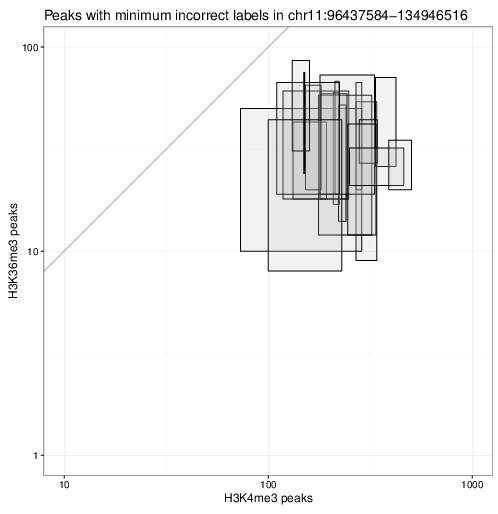
\includegraphics[width=0.7\textwidth]{figure-min-err-peaks-compare}
\end{frame}

\begin{frame}
  \frametitle{Smaller peaks in sharp H3K4me3 than in broad H3K36me3}
  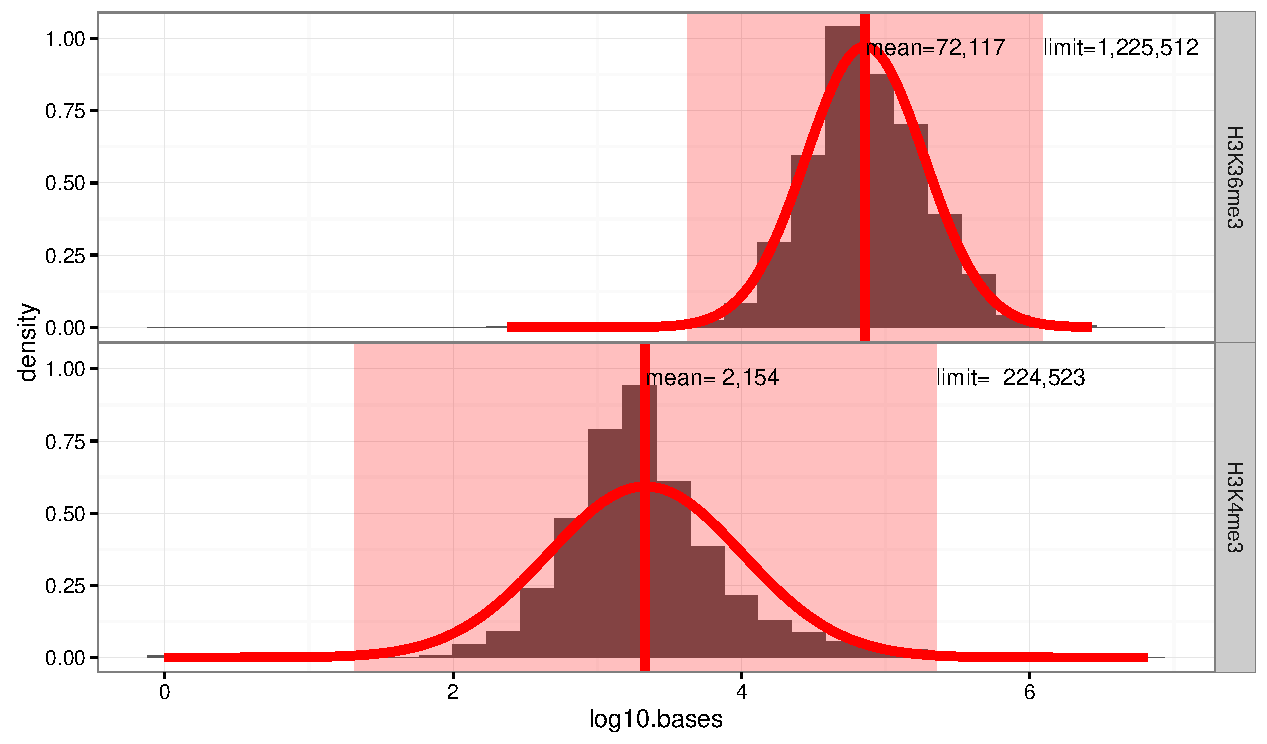
\includegraphics[width=\textwidth]{figure-peak-size-model}
\end{frame}

\begin{frame}
  \frametitle{Only need 10--25 runs to find optimal penalty interval}
  \includegraphics[width=0.8\textwidth]{figure-timing-data-penalties}
\end{frame}

\begin{frame}
  \frametitle{Target interval computation time}
  \includegraphics[width=\textwidth]{figure-target-interval-time}
\end{frame}

\begin{frame}
  \frametitle{Pipeline}
Input:
\begin{itemize}
\item $S$ bigWig coverage data files, 
\item problems.bed file with $P$ genomic regions to segment, 
\item labels.txt file(s) -- gold standard locations with and without peaks.
\end{itemize}
For example $S=37$ samples, $P=374$ problems in hg19.
\vskip 0.2cm
  \begin{tabular}{lrr}
    Step& Jobs& Time/job \\
    \hline
    Create separate problems & 1 & 5 min\\
    Compute separate targets & $S P$ & 1--10 hours\\
    Train separate model & 1 & 5 min \\
    Separate peak prediction & $P$ & 1--10 hours\\
    Train joint model & 1 & 5 min \\
    Joint peak prediction & $P$ & 1--10 hours\\
    Combine and plot predictions & 1 & 10--60 minutes
  \end{tabular}
\vskip 0.2cm
Output: matrix of joint peak predictions, samples x peaks.
\end{frame}

\section{Conclusions and future work}

\begin{frame}[fragile]
  \frametitle{How to choose parameters of unsupervised peak
    detectors?}
\scriptsize
19 parameters for Model-based analysis of ChIP-Seq (MACS), Zhang et al, 2008.
\begin{verbatim}
  [-g GSIZE]
  [-s TSIZE] [--bw BW] [-m MFOLD MFOLD] [--fix-bimodal]
  [--nomodel] [--extsize EXTSIZE | --shiftsize SHIFTSIZE]
  [-q QVALUE | -p PVALUE | -F FOLDENRICHMENT] [--to-large]
  [--down-sample] [--seed SEED] [--nolambda]
  [--slocal SMALLLOCAL] [--llocal LARGELOCAL]
  [--shift-control] [--half-ext] [--broad]
  [--broad-cutoff BROADCUTOFF] [--call-summits]
\end{verbatim}
10 parameters for Histone modifications in cancer (HMCan),
Ashoor et al, 2013.
\begin{verbatim}
minLength 145
medLength 150
maxLength 155
smallBinLength 50
largeBinLength 100000
pvalueThreshold 0.01
mergeDistance 200
iterationThreshold 5
finalThreshold 0
maxIter 20
\end{verbatim}
\end{frame}

\begin{frame}
  \frametitle{PeakSeg: search for the peaks with lowest loss}
  \includegraphics[width=1\textwidth]{figure-macs-problem-PeakSeg.png}
  
  Simple model with only one parameter to train (maxPeaks).
\end{frame}

\begin{frame}
  \frametitle{Conclusions}
  \begin{tabular}{r|c|c}
    & no pruning & functional pruning \\
    \hline
    unconstrained & Dynamic Programming & PDPA, FPOP \\
     & exact $O(N^2)$ & exact $O(N\log N)$\\
    R packages: & changepoint & cghseg, Segmentor\\
    \hline
    up-down constrained & constrained DP & \textbf{this work} \\
     & inexact $O(N^2)$ & exact $O(N\log N)$\\
    R packages: & PeakSegDP & \textbf{coseg}\\
    \hline
  \end{tabular}
  \begin{itemize}
  \item New algorithm that \textbf{exactly} computes the
    \textbf{constrained} optimal change-points/peaks for $N$ data points.
  \item C++ code in coseg R package, $O(N \log N)$ memory
    \url{https://github.com/tdhock/coseg}
  \item PeakSegFPOP program for big $N > 10^6$ data,
    $O(\log N)$ memory and $O(N\log N)$ disk space.
  \item TODO: ICML paper.
  \item TODO: C3G-GSOC pipeline project.
  \item TODO: web app for interactive labeling and model learning.
  \end{itemize}
\end{frame}

\begin{frame}
  \frametitle{Thanks for your attention!}

  Questions? toby.hocking@mail.mcgill.ca
  \begin{itemize}
  \item 
  \textbf{coseg} R package, \\
  \url{https://github.com/tdhock/coseg}
  \item 
    \textbf{PeakSegFPOP} command line program, 
  \url{https://github.com/tdhock/PeakSegFPOP}
  \item source code for these slides:
  \url{https://github.com/tdhock/PeakSegFPOP-paper}
  \end{itemize}
\end{frame}

\begin{frame}
  \frametitle{Two annotators provide consistent labels, but different
    precision}
  \includegraphics[width=1.1\textwidth]{../chip-seq-paper/screenshot-several-annotators}

  \begin{itemize}
  \item TDH peakStart/peakEnd more precise than AM peaks.
  \item AM noPeaks more precise than TDH no label.
  \end{itemize}
\end{frame}

\begin{frame}
  \frametitle{Train on one person, test on another\\
(same histone mark and samples)}
  \includegraphics[width=1\textwidth]{../chip-seq-paper/figure-splits-H3K4me3-annotators.pdf}
\end{frame}

\begin{frame}
  \frametitle{Train on one person, test on another\\
(same histone mark and samples)}
  \includegraphics[width=1.1\textwidth]{../chip-seq-paper/figure-test-H3K4me3-annotators.pdf}
\end{frame}

\begin{frame}
  \frametitle{Train on some samples, test on others\\
(same histone mark and person)}
  \includegraphics[width=1\textwidth]{../chip-seq-paper/figure-splits-H3K4me3-types.pdf}
\end{frame}

\begin{frame}
  \frametitle{Train on some samples, test on others\\
(same histone mark and person)}
  \includegraphics[width=1.1\textwidth]{../chip-seq-paper/figure-test-H3K4me3-types.pdf}
\end{frame}

\begin{frame}
  \frametitle{Train on one histone mark, test on another\\
(same person and samples)}
  \includegraphics[width=1\textwidth]{../chip-seq-paper/figure-splits-TDH-experiments.pdf}
\end{frame}

\begin{frame}
  \frametitle{Train on one histone mark, test on another\\
(same person and samples)}
  \includegraphics[width=1.1\textwidth]{../chip-seq-paper/figure-test-TDH-experiments.pdf}
\end{frame}

\end{document}
